\documentclass{article}

\usepackage{amsmath, amsthm, amssymb, amsfonts}
\usepackage{thmtools}
\usepackage{graphicx}
\usepackage{setspace}
\usepackage{geometry}
\usepackage{float}
\usepackage{hyperref}
\usepackage[utf8]{inputenc}
\usepackage[english]{babel}
\usepackage{framed}
\usepackage[dvipsnames]{xcolor}
\usepackage{tcolorbox}
\usepackage{multirow}
\usepackage{tabularx}
\usepackage{longtable}
\usepackage{fancyhdr}
\usepackage{listings}


% Other
\usepackage{algorithmic}
\usepackage{array}
\usepackage[caption=false,font=footnotesize]{subfig}
\usepackage{lipsum}
\usepackage{hyperref}


% ------------------------------------------------------------------------------
% Name, Course Code and Date
% ------------------------------------------------------------------------------

\newcommand{\name}{Group 4}
\newcommand{\idnumber}{00000000}
\newcommand{\coursecode}{COMP3017J}
\newcommand{\paperdate}{\today}

% ------------------------------------------------------------------------------


\pagestyle{fancy}
\newlength\FHoffset
\setlength\FHoffset{0.1cm}

\addtolength\headwidth{2\FHoffset}
\fancyhead[L]{\name}
\fancyhead[C]{\coursecode}
\fancyhead[R]{\paperdate}



\colorlet{LightGray}{White!90!Periwinkle}
\colorlet{LightOrange}{Orange!15}
\colorlet{LightGreen}{Green!15}

\newcommand{\HRule}[1]{\rule{\linewidth}{#1}}

\declaretheoremstyle[name=Theorem,]{thmsty}
\declaretheorem[style=thmsty,numberwithin=section]{theorem}
\tcolorboxenvironment{theorem}{colback=LightGray}

\declaretheoremstyle[name=Proposition,]{prosty}
\declaretheorem[style=prosty,numberlike=theorem]{proposition}
\tcolorboxenvironment{proposition}{colback=LightOrange}

\declaretheoremstyle[name=Principle,]{prcpsty}
\declaretheorem[style=prcpsty,numberlike=theorem]{principle}
\tcolorboxenvironment{principle}{colback=LightGreen}

\setstretch{1.2}
\geometry{
    textheight=9in,
    textwidth=6.0in,
    top=1in,
    headheight=12pt,
    headsep=25pt,
    footskip=30pt
}

\usepackage{listings}
\lstset{ %
language=C++,                % choose the language of the code
basicstyle=\footnotesize,       % the size of the fonts that are used for the code
numbers=left,                   % where to put the line-numbers
numberstyle=\footnotesize,      % the size of the fonts that are used for the line-numbers
stepnumber=1,                   % the step between two line-numbers. If it is 1 each line will be numbered
numbersep=5pt,                  % how far the line-numbers are from the code
backgroundcolor=\color{white},  % choose the background color. You must add \usepackage{color}
showspaces=false,               % show spaces adding particular underscores
showstringspaces=false,         % underline spaces within strings
showtabs=false,                 % show tabs within strings adding particular underscores
frame=single,           % adds a frame around the code
tabsize=2,          % sets default tabsize to 2 spaces
captionpos=b,           % sets the caption-position to bottom
breaklines=true,        % sets automatic line breaking
breakatwhitespace=false,    % sets if automatic breaks should only happen at whitespace
escapeinside={\%*}{*)}          % if you want to add a comment within your code
}

% ------------------------------------------------------------------------------

\begin{document}

% ------------------------------------------------------------------------------
% Cover Page and ToC
% ------------------------------------------------------------------------------

\title{ \normalsize  
\includegraphics[width=0.1\textwidth]{images/UCD_Logo.pdf} \textbf{ }

\includegraphics[width=0.15\textwidth]{images/BJUT_Logo.pdf} \par \textsc{Beijing-Dublin International College}
		\\ [2.0cm]
		\HRule{1.5pt} \\ [0.35cm]
		\LARGE \textbf{\uppercase{\coursecode \ Software Methodology Project Report}}
		\HRule{1.5pt} \\ [0.9cm] \textbf{\LARGE{OuterView: An Online Technical Interview Platform}} \vspace*{6\baselineskip}
		}
\date{\paperdate}
\author{\textbf{Authors} \\ 
  Jiehongxu Wu (21372323) \\
  Sichen Li (21372309) \\
  Te Qi (21372325) \\
  Tongyu Wu (21372320) \\
  Ziqin Ma (21372329)
}

\maketitle
\newpage

\tableofcontents
\newpage

% ------------------------------------------------------------------------------

\section{Preface}

The intended readers of this document are primarily technical interviewing platform developers, 
product managers, and other stakeholders involved in the design, development, and implementation 
of collaborative technical interviewing software systems. The purpose of this document is to 
provide a comprehensive overview of the system requirements and customer problem statement, 
clearly defining the requirements and capabilities of the platform to guide the development team 
in creating solutions that meet the needs of interviewers and candidates.

This document has gone through several versions, each improving and expanding on the previous 
version. The rationale for creating a new version is to incorporate stakeholder feedback, update 
the document with the latest requirements, and improve overall clarity and organization.

A summary of the changes made in each release is as follows:

\begin{itemize}
    \item Version 1.0
    \begin{enumerate}
        \item Initial version of the document. Provided an overview of the system requirementsof the technical interview platform.
        \item Identifed customer problem statements and software system recommendations to solve problems faced by customers.
    \end{enumerate}
    \item Version 1.1
    \begin{enumerate}
        \item The description of the problem statement was enhanced to include more examples and details, and stakeholder feedback was incorporated to further refine the content and requirements to illustrate the customer challenges.
        \item Drew use case diagrams and completed use case descriptions to improve the accuracy of project understanding.
        \item Completed the user requirements definition part to make the project requirements clearer.
    \end{enumerate}
    \item Version 1.2
    \begin{enumerate}
        \item A preface has been added to identify the intended readership and provide context for the document.
        \item A glossary of terms was completed to clarify concepts related to professional terms used in the project.
        \item Completed the UI design and production of the front-end main page, reservation meeting page, and meeting information page.
        \item Implemented the backend logic related to sign up, login and reservation meeting and completed the corresponding database design.
        \item Build the project foundation.
    \end{enumerate}
    \item Version 1.3
    \begin{enumerate}
        \item Completed system requirements definition.
        \item Updated document structure to improve organization and readability.
        \item The front-end and back-end implementation of login registration function.
        \item Further improvements in the backend to meet the need of frontend.
        \item Completed the rendering and basic logic of the frontend main page, reservation meeting page, and meeting information page.
    \end{enumerate}
    \item Version 1.4
    \begin{enumerate}
        \item Completed an interaction diagram primarily based on sequence diagrams and a class diagram.
        \item Completed interface specification related content.
        \item Created partial content on system architecture and system design.
        \item Completed the layout and style of the meeting room page, and integrated IDE and RTC.
        \item Completed the front-end and partial back-end implementation of the IDE page.
        \item Completed partial implementation of video calls.
    \end{enumerate}
    \item Version 1.5
    \begin{enumerate}
        \item Completed all aspects of system architecture and design.
        \item Understood and completed the content of algorithms and data structures.
        \item Completed the code implementation for video calls.
        \item Completed all code implementations for the IDE page.
    \end{enumerate}
    \item Version 1.6
    \begin{enumerate}
        \item Completed the overall requirements of the project.
        \item Completed all parts of the test cases and synchronized the refinement of the terminology to avoid potential ambiguity issues.
        \item A comprehensive review and revision of the project report was conducted.
        \item Each version of this document has been carefully prepared to provide a comprehensive and up-to-date overview of the technical interview platform requirements and customer question statements. The current version 1.6 is the most detailed and accurate representation of system requirements and objectives.
    \end{enumerate}
\end{itemize}


\section{System Specification}
\subsection{Customer Problem Statement}

As a customer, I am facing the problem of conducting technical interviews in an inefficient and time-consuming manner. Traditional interview methods often involve face-to-face meetings, which can be challenging due to time constraints, geographical limitations, and the need for specialized equipment. For instance, scheduling interviews with candidates from different time zones or remote locations can be difficult, and setting up a suitable environment for coding tasks can be expensive and time-consuming. Additionally, it can be difficult to accurately evaluate a candidate’s skills and knowledge without a proper platform for live collaboration and code execution.

To address these challenges, I suggest a software system that provides a live, collaborative environment for both interviewers and candidates to write, execute, and debug code together. This system should help candidates easily share their skills and support multiple programming languages, such as Python, JavaScript, and Java. It should also have video and audio interviewing functions, scheduling and management features for interviewers, a virtual whiteboard, and the ability to evaluate a candidate’s code with automated test cases. Additionally, the system should allow me to replay interviews for future reference, helping me to better assess candidate performance and make more informed decisions.

By implementing this software system, I believe it will significantly improve the efficiency and effectiveness of technical interviews, enabling me to identify the best candidates more quickly and accurately. This will not only save time and resources but also enhance the overall quality of the interview process, leading to better matches between candidates and employers.

\subsection{Glossary of Terms}

\begin{itemize}
  \item \textbf{Technical Interview Platform:} A website designed to facilitate live, collaborative technical interviews between interviewers and candidates. 
  \item \textbf{Browser-based IDE:} A web-based integrated development environment that allows candidates to share their coding skills during interviews. 
  \item \textbf{Programming Language:} A set of rules and conventions used to create computer programs. 
  \item \textbf{Video and Audio Interviewing:} Functionality that allows interviewers and candidates to communicate via video and audio during the interview process. 
  \item \textbf{Scheduling and Management:} Features that enable interviewers to schedule and manage interviews efficiently. 
  \item \textbf{Virtual Whiteboard:} A digital whiteboard that allows interviewers and candidates to visualize their technical conversations during interviews. 
  \item \textbf{Automated Test Cases:} Pre-written tests that evaluate a candidate’s code for correctness and efficiency. 
  \item \textbf{Playback Function:} A feature that allows interviewers to replay the entire interview after it has ended. 
  \item \textbf{Not Start:} The meeting has not yet started, and the interviewee is waiting for the meeting.
  \item \textbf{In progress:} The meeting is currently in progress, and the interviewees are in the meeting status.
  \item \textbf{Completed:} The meeting has ended, and the interview is now in its current state.
\end{itemize}


\subsection{User Requirements Definition}

% \begin{tabular}{ |p{1cm}||p{2.3cm}|p{9cm}|  }
%     \hline
%     \multicolumn{3}{|c|}{Requirements List} \\
%     \hline
%     Priority& Type &Description\\
%     \hline
%     1 & Functional\par Requirements  &Both interviewers and interviewees can see the meeting arrangement in chronological order downwards at the bottom of the homepage.\\
%     1 &  Functional\par Requirements  & Interviewers can initiate audio and video calls or pure audio calls with other designated users. \\
%     1 &  Functional\par Requirements  & Interviewers can cancel a meeting\\
%     1 &  Functional\par Requirements  & Both interviewers and interviewees can set a reminder for their meetings.\\
%     1 &  Functional\par Requirements  & Both interviewers and interviewees can end the meeting session.\\
%     1 &  Functional\par Requirements  & Both interviewers and interviewees can re-enter the meeting session they leave as long as the other users in the meeting remain in the session. \\
%     1 &  Functional\par Requirements  & Both interviewers and interviewees can choose which microphone and camera they use for meetings.\\
%     1 &  Functional\par Requirements  & Both interviewers and interviewees can choose different programming languages for coding in the meeting.\\
%     1 &  Functional\par Requirements  & Both interviewers and interviewees can run the code in the editor and debug them..\\
%     1 &  Functional\par Requirements  & Both interviewers and interviewees can comment and change the code in the editor.\\
%     1 &  Functional\par Requirements  & Interviewers can set the questions and send them to the interviewees..\\
%     1 &  Functional\par Requirements  & Interviewers can send answers to the interviewees.\\
%     1 &  Non-Functional\par Requirements  & Interviewers can set a timer for the session and each question.\\
%     1 &  User Interface\par Requirements  & Both interviewers and interviewees have buttons for booking meetings and joining meetings on the homepage.\\
%     1 &  User Interface\par Requirements  & Interviewers have a button for canceling or changing a meeting in the meeting list on the homepage.\\
%     1 &  User Interface\par Requirements  & Both interviewers and interviewees can see tags containing the name, start time, organizer for each booked meeting in the list on the homepage.\\
%     1 &  User Interface\par Requirements  & Both interviewers and interviewees can see the reminder they set for the meeting in the list on the homepage.\\
%     1 &  User Interface\par Requirements  & Interviewers have buttons for canceling and changing the meeting in the meeting session.\\
%     1 &  User Interface\par Requirements  & Both interviewers and interviewees have a button for exiting from the current page in the meeting session.\\
%     1 &  User Interface\par Requirements  & Both interviewers and interviewees can see the ID and title of the meeting and the username and position of all the users in the meeting session.\\
%     1 &  User Interface\par Requirements  & Both interviewers and interviewees can see the viewing frame of their camera and the other sides' and change the size of all these frames.\\

%     \hline
%    \end{tabular}

 
%  \begin{longtable}{ |p{1cm}||p{2.3cm}|p{9cm}|  }

%  \hline
%  \multicolumn{3}{| c |}{Requirements List}\\
%  \hline
%  \endfirsthead

%  \hline
%  Priority& Type &Description\\
%  \hline
%  1 & Functional\par Requirements  &Both interviewers and interviewees can see the meeting arrangement in chronological order downwards at the bottom of the homepage.\\
%  \hline
%  1 &  Functional\par Requirements  & Interviewers can initiate audio and video calls or pure audio calls with other designated users. \\
%  \hline
%  1 &  Functional\par Requirements  & Interviewers can cancel a meeting\\
%  \hline
%  1 &  Functional\par Requirements  & Both interviewers and interviewees can set a reminder for their meetings.\\
%  \hline

%  1 &  Functional\par Requirements  & Both interviewers and interviewees can end the meeting session.\\
%  \hline

%  1 &  Functional\par Requirements  & Both interviewers and interviewees can re-enter the meeting session they leave as long as the other users in the meeting remain in the session. \\
%  \hline

%  1 &  Functional\par Requirements  & Both interviewers and interviewees can choose which microphone and camera they use for meetings.\\
%  \hline

%  1 &  Functional\par Requirements  & Both interviewers and interviewees can choose different programming languages for coding in the meeting.\\
%  \hline

%  1 &  Functional\par Requirements  & Both interviewers and interviewees can run the code in the editor and debug them..\\
%  \hline

%  1 &  Functional\par Requirements  & Both interviewers and interviewees can comment and change the code in the editor.\\
%  \hline
%  1 &  Functional\par Requirements  & Interviewers can set the questions and send them to the interviewees..\\
%  \hline
%  1 &  Functional\par Requirements  & Interviewers can send answers to the interviewees.\\
%  \hline
%  1 &  Non-Functional\par Requirements  & Interviewers can set a timer for the session and each question.\\
%  \hline
%  1 &  User Interface\par Requirements  & Both interviewers and interviewees have buttons for booking meetings and joining meetings on the homepage.\\
%  \hline
%  1 &  User Interface\par Requirements  & Interviewers have a button for canceling or changing a meeting in the meeting list on the homepage.\\
%  \hline
%  1 &  User Interface\par Requirements  & Both interviewers and interviewees can see tags containing the name, start time, organizer for each booked meeting in the list on the homepage.\\
%  \hline
%  1 &  User Interface\par Requirements  & Both interviewers and interviewees can see the reminder they set for the meeting in the list on the homepage.\\
%  \hline
%  1 &  User Interface\par Requirements  & Interviewers have buttons for canceling and changing the meeting in the meeting session.\\
%  \hline
%  1 &  User Interface\par Requirements  & Both interviewers and interviewees have a button for exiting from the current page in the meeting session.\\
%  \hline
%  1 &  User Interface\par Requirements  & Both interviewers and interviewees can see the ID and title of the meeting and the username and position of all the users in the meeting session.\\
%  \hline
%  1 &  User Interface\par Requirements  & Both interviewers and interviewees can see the viewing frame of their camera and the other sides' and change the size of all these frames.\\

%  \hline
%  \end{longtable}

\begin{longtable}{ |p{1cm}||p{2.3cm}|p{9cm}|  }
 

  \hline
  \multicolumn{3}{| c |}{Requirements List}\\
  \hline
  \endfirsthead
 
 
  \hline
  Priority& Type &Description\\
  \hline
  10 & Functional\par Requirements  &Both interviewers and interviewees can see the meeting arrangement in chronological order downwards at the bottom of the homepage.\\
  \hline
  10 &  Functional\par Requirements  & Interviewers can initiate audio and video calls or pure audio calls with other designated users. \\
  \hline
  10 &  Functional\par Requirements  & Interviewers can cancel a meeting\\
  \hline
  5 &  Functional\par Requirements  & Both interviewers and interviewees can set a reminder for their meetings.\\
  \hline
 
  10 &  Functional\par Requirements  & Both interviewers and interviewees can end the meeting session.\\
  \hline
 
  8 &  Functional\par Requirements  & Both interviewers and interviewees can re-enter the meeting session they leave as long as the other users in the meeting remain in the session. \\
  \hline
 
  5 &  Functional\par Requirements  & Both interviewers and interviewees can choose which microphone and camera they use for meetings.\\
  \hline
 
  5 &  Functional\par Requirements  & Both interviewers and interviewees can choose different programming languages for coding in the meeting.\\
  \hline
 
  8 &  Functional\par Requirements  & Both interviewers and interviewees can run the code in the editor and debug them..\\
  \hline
 
  5 &  Functional\par Requirements  & Both interviewers and interviewees can comment and change the code in the editor.\\
  \hline
  8 &  Functional\par Requirements  & Interviewers can set the questions and send them to the interviewees..\\
  \hline
  5 &  Functional\par Requirements  & Interviewers can send answers to the interviewees.\\
  \hline
  3 &  Non-Functional\par Requirements  & Interviewers can set a timer for the session and each question.\\
  \hline
  10 &  User Interface\par Requirements  & Both interviewers and interviewees have buttons for booking meetings and joining meetings on the homepage.\\
  \hline
  8 &  User Interface\par Requirements  & Interviewers have a button for canceling or changing a meeting in the meeting list on the homepage.\\
  \hline
  8 &  User Interface\par Requirements  & Both interviewers and interviewees can see tags containing the name, start time, organizer for each booked meeting in the list on the homepage.\\
  \hline
  3 &  User Interface\par Requirements  & Both interviewers and interviewees can see the reminder they set for the meeting in the list on the homepage.\\
  \hline
  3 &  User Interface\par Requirements  & Interviewers have buttons for canceling and changing the meeting in the meeting session.\\
  \hline
  10 &  User Interface\par Requirements  & Both interviewers and interviewees have a button for exiting from the current page in the meeting session.\\
  \hline
  10 &  User Interface\par Requirements  & Both interviewers and interviewees can see the ID and title of the meeting and the username and position of all the users in the meeting session.\\
  \hline
  8 &  User Interface\par Requirements  & Both interviewers and interviewees can see the viewing frame of their camera and the other sides' and change the size of all these frames.\\
 
  \hline
  \end{longtable}


   \subsection{System Requirements Specification}
   \subsubsection*{Stakeholders}
   The stakeholders of the system are the interviewers and interviewees who need to conduct the programming interview. In our case, the interviewer and the interviewee can set up a meeting, so that the interviewer can see the interviewee's programming situation in real time, and make comments and code compilation in real time. The interviewee will also be able to see the interviewer's comments in real time and will be able to communicate via video.
   \subsubsection*{Actors and Goals}
   \begin{tabular}{ |p{3cm}||p{6.5cm}|  }
    \hline
    \multicolumn{2}{|c|}{Actors and Goals List} \\
    \hline
    Actors & Goals\\
    \hline
    Interviewers   & Registration and login\\
    Interviewers   & Schedule or cancel a meeting\\
    Interviewers   & Join or exit a meetingn\\
    Interviewers   & Ability to compile and run code\\
    Interviewers   & Ability to write comments\\
    Interviewers   & Turn on/off microphone and camera\\
    Interviewees   & Registration and login\\
    Interviewees   & Join or exit a meeting\\
    Interviewees   & Ability to compile and run code\\
    Interviewees   & Ability to write comments\\
    Interviewees   & Turn on/off microphone and camera\\
    Interviewees   & Ability to choose programming language\\
    \hline
   \end{tabular}

   \subsubsection*{User Cases}
   \textbf{User Case Diagram: }

   \begin{figure}[H]
    \centering
    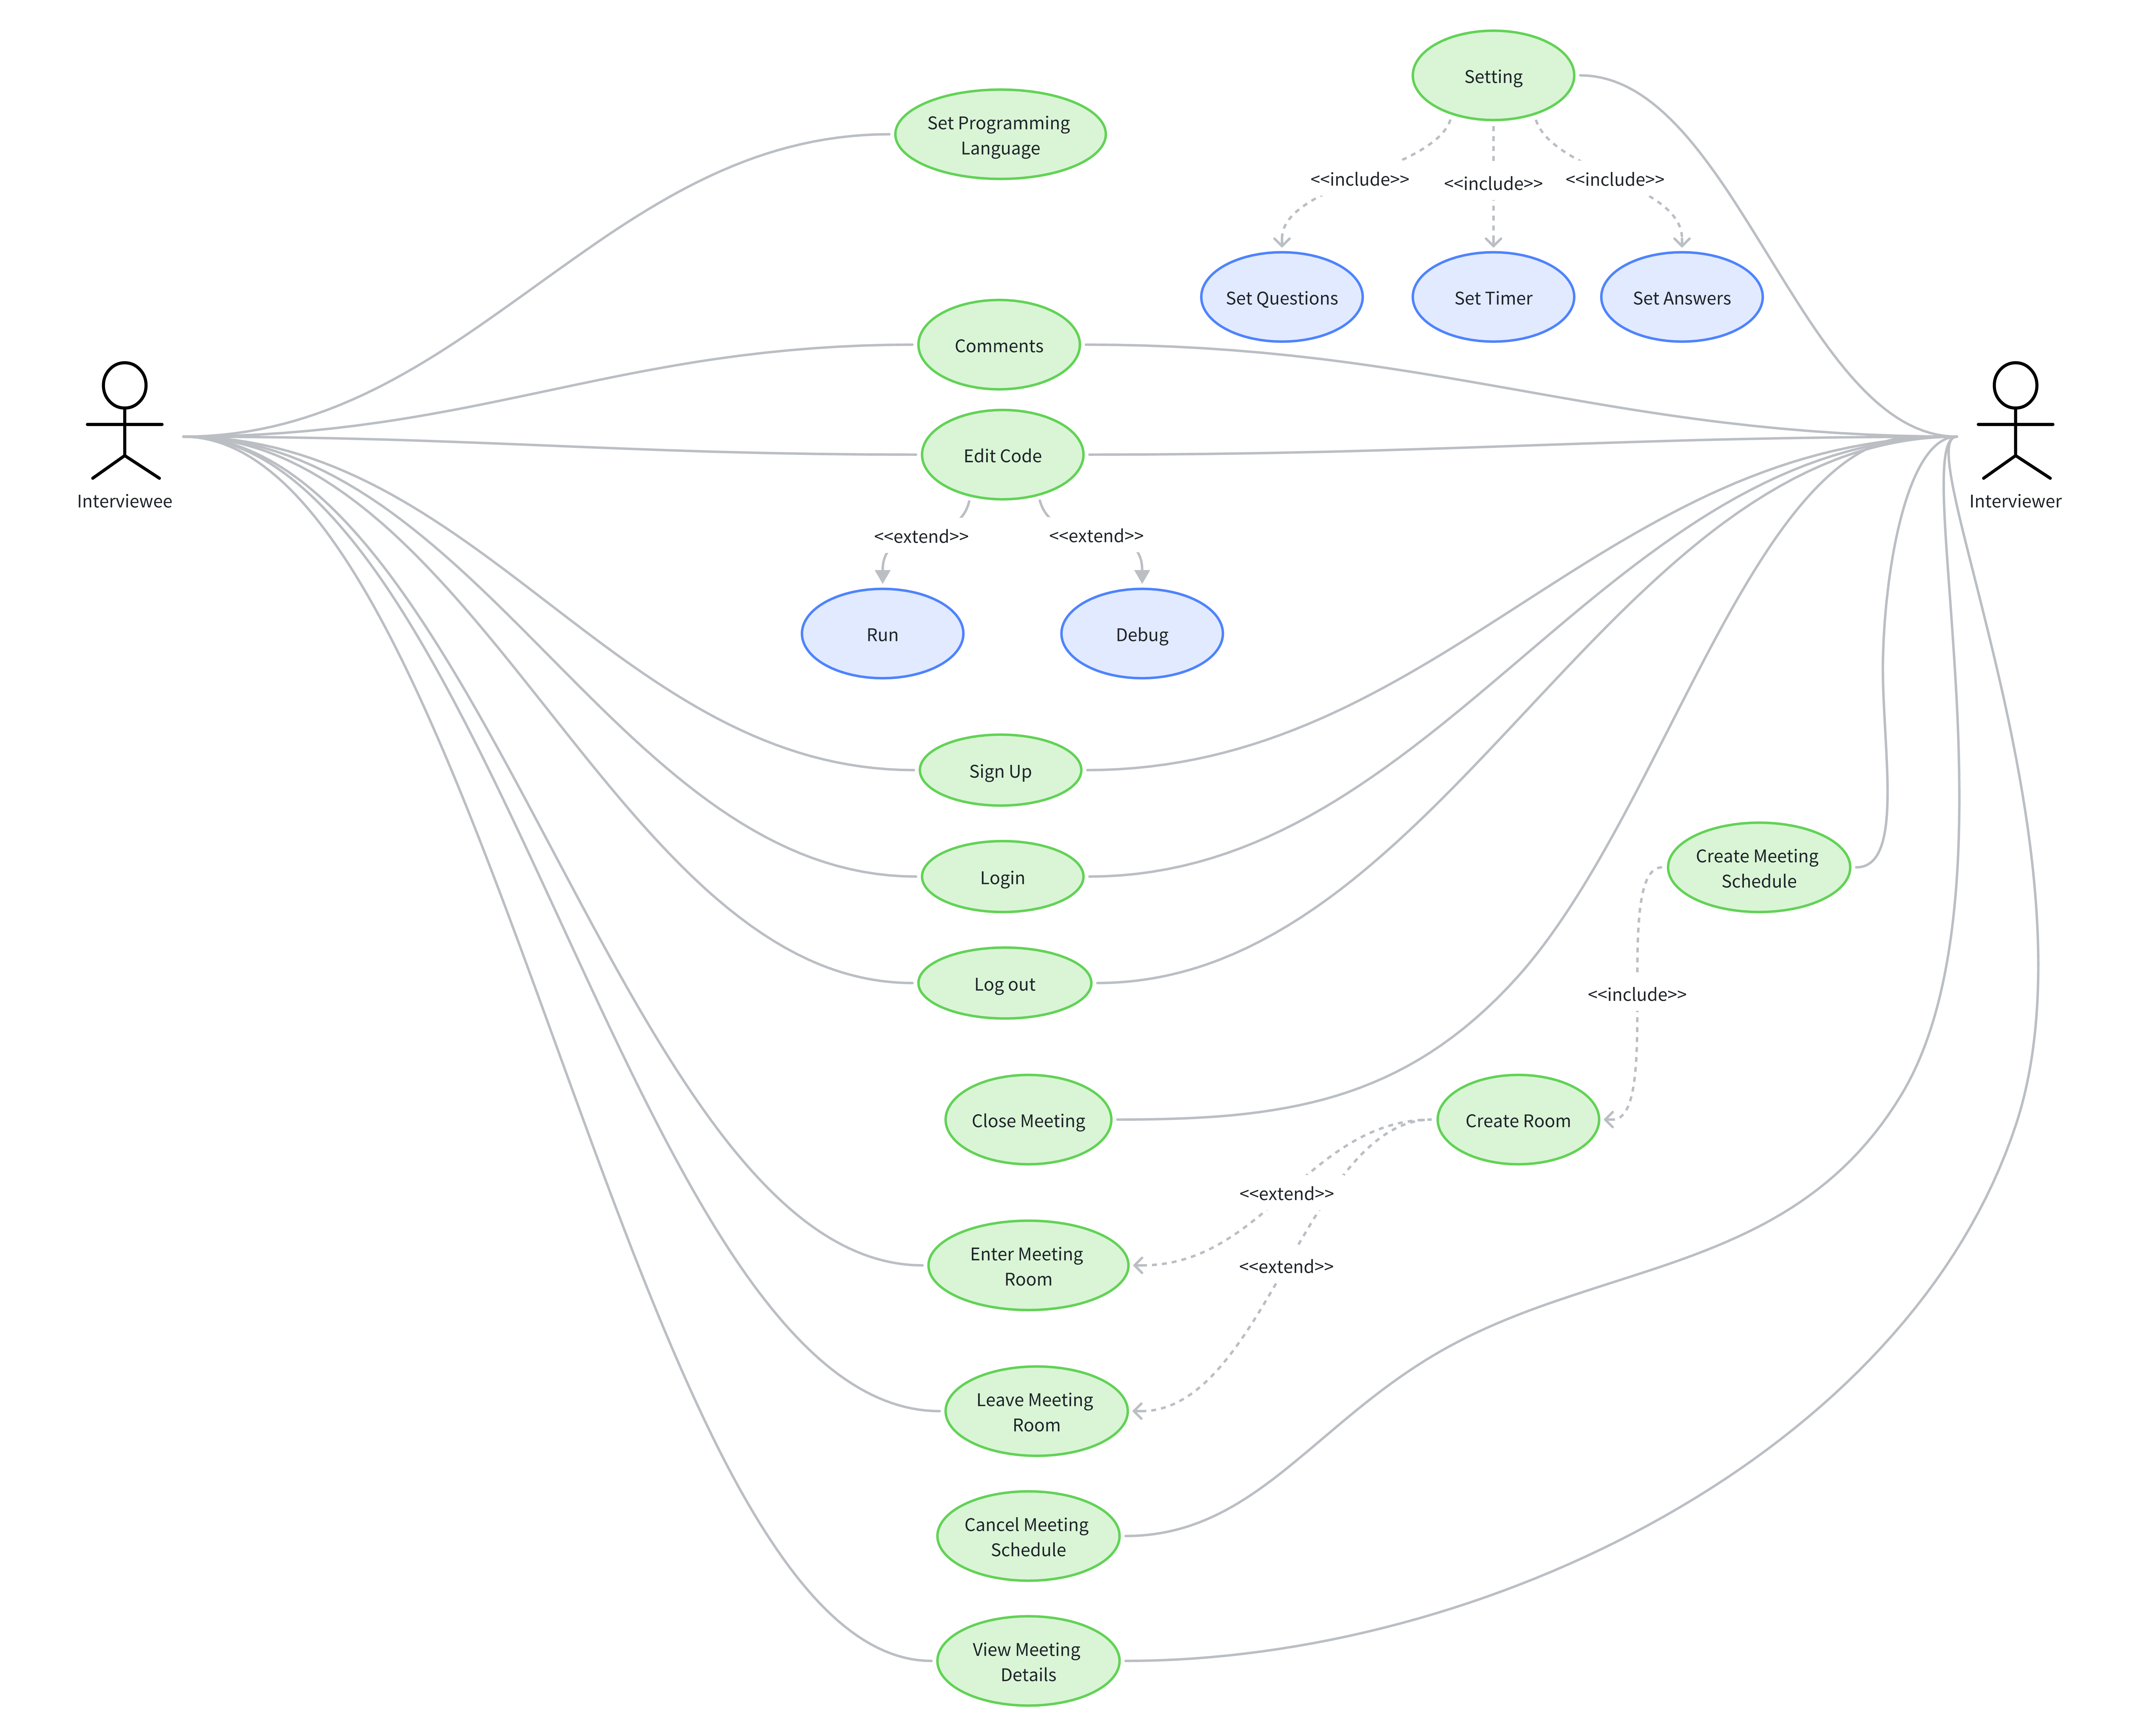
\includegraphics[scale=0.065]{diagrams/use-case-diagram.png}
    \caption{Use Case Diagram}
\end{figure}
\newpage

   \textbf{Casual Description: }
   \begin{itemize}
    \item \textbf{UC1:} \par \textbf{Sign Up:} Users can create new accounts.
    \item \textbf{UC2:} \par \textbf{Login:} Users can login using the registered account.
    \item \textbf{UC3:} \par \textbf{Log out:} Users can exit the current account.
    \item \textbf{UC4:} \par \textbf{Enter Meeting Room:} Users can enter the meeting.
    \item \textbf{UC5:} \par \textbf{Leave Meeting Room:} Users can leave the meeting.
    \item \textbf{UC6:} \par \textbf{Create Meeting Schedule:} Interviewers can create new meeting schedule.
    \item \textbf{UC7:} \par \textbf{Cancel Meeting Schedule:} Interviewers can cancel a meeting schedule.
    \item \textbf{UC8:} \par \textbf{View Meeting Details:} Users can see the details of a scheduled meeting.
    \item \textbf{UC9:} \par \textbf{Create Room:} Interviewers can create new meeting rooms.
    \item \textbf{UC10:} \par \textbf{Close Meeting:} Interviewers can end the meeting rooms.
    \item \textbf{UC11:} \par \textbf{Set Programming Language:} Interviewees can choose a programming language.
    \item \textbf{UC12:} \par \textbf{Setting:} Interviewers are able to set interview questions, answers, answer times, etc.
    \item \textbf{UC13:} \par \textbf{Edit Code:} Interviewees can edit code, run and debug code.
    \item \textbf{UC14:} \par \textbf{Comments:} Users can write comments.
    \item \textbf{UC15:} \par \textbf{Set Questions:} Interviewers can set questions.
    \item \textbf{UC16:} \par \textbf{Set Timer:} Interviewers can set a timer for the interviewees in a timed question.
    \item \textbf{UC17:} \par \textbf{Set Answers:} Interviewers can set answers for the questions they set.

   \end{itemize}

   \textbf{Detailed User Case Descriptions: }\par

   \begin{tabularx}{0.9\textwidth} { 
    | >{\raggedright\arraybackslash}X 
    | >{\centering\arraybackslash}X | }
   \hline
   \textbf{Use Case UC1: Sign Up} \\
   \hline
   \textbf{Summary:} Describes how the user successfully goes to the home page. \\
   \hline
   \textbf{Precondition:} The Sign Up page must be open in a browser meeting the system requirements.\\
   \hline
   \textbf{Trigger:} mouse click\\
   \hline
   \textbf{Event Process:}
   \begin{enumerate}
    \item The user will be prompted to enter an user name, user id, email and password.
    \item The user inputs the information.
    \item The user clicks "Sign Up Now" button to register an account.
   \end{enumerate}\\
   \hline
  \end{tabularx}

   \begin{tabularx}{0.9\textwidth} { 
    | >{\raggedright\arraybackslash}X 
    | >{\centering\arraybackslash}X | }
   \hline
   \textbf{Use Case UC4: Enter Meeting Room} \\
   \hline
   \textbf{Summary:} The user (interviewer and/or interviewee) can join the meeting room, start the interview, choose to turn on/off the camera and microphone, open the shared IDE, and exit the meeting room \\
   \hline
   \textbf{Precondition:} The user is added to the meeting room by the interviewer. The meeting room is available on the user's home page.\\
   \hline
   \textbf{Trigger:} mouse click\\
   \hline
   \textbf{Event Process:}
   \begin{enumerate}
    \item The user clicks the "Enter Meeting Room" button next to the meeting room to connect to the meeting room.
    \item Users enable the camera and microphone (off by default).
    \item The screen displays the screen status, microphone status, name and other information of other users in the meeting room.
    \item Start the interview.
    \item Click Share IDE to share the IDE with others in the meeting room.
   \end{enumerate}\\
   \hline
  \end{tabularx}

  \begin{tabularx}{0.9\textwidth} { 
    | >{\raggedright\arraybackslash}X 
    | >{\centering\arraybackslash}X | }
   \hline
   \textbf{User Case UC6: Create Meeting Schedule:} \\
   \hline
   \textbf{Summary:} Users can create meetings.\\
   \hline
   \textbf{Precondition:} The main window must be open in a browser meeting the system requirements.\\
   \hline
   \textbf{Trigger:} mouse click\\
   \hline
   \textbf{Event Process:}
   \begin{enumerate}
    \item If the user wants to create a meeting, click "Create Meeting Schedule".
    \item Users need to fill in more information for this meeting in the display section. Information to fill in may includes:
    \begin{itemize}
        \item Meeting name (default name is username)
        \item Start time and end time
        \item Duration of the meeting (30min, 45min and 60min for option)
        \item Participants of the meeting
    \end{itemize}
    \item Users invited to the meeting. This field requires an ID.
    \item The user clicks "Complete appointment" below the display section to finish filling the information.
    \item After completion, the user will return to the main page and see the newly scheduled meeting in the right scheduling table.
   \end{enumerate}\\
   \hline
  \end{tabularx}

  \begin{tabularx}{0.9\textwidth} { 
    | >{\raggedright\arraybackslash}X 
    | >{\centering\arraybackslash}X | }
   \hline
   \textbf{User Case UC8: View Meeting Details:} \\
   \hline
   \textbf{Summary:} The user can see the details about a meeting.\\
   \hline
   \textbf{Precondition:} The user has the meeting he or she wants to attend scheduled.\\
   \hline
   \textbf{Trigger:} mouse click\\
   \hline
   \textbf{Event Process:}
   \begin{enumerate}
    \item In the configuration table on the right, click the meeting for which the user wants to view specific information.
    \item The page will provide a pop-up window to show the details of the meeting. The information displayed may include:
    \begin{itemize}
        \item Meeting name (default name is username)
        \item Start time and end time
        \item Duration of the meeting (30min, 45min and 60min for option)
        \item Participants of the meeting
    \end{itemize}
    \item The user clicks "Enter Meeting" in the pop-up window to complete the request; or click the "Back" button in the upper left corner to close the popup.
    \item The "Cancel Meeting" and "Edit Meeting" buttons at the bottom of the pop-up window are only eligible for the people who create the meeting schedule to click; the invitees cannot click either button. After clicking "Cancel Meeting", the meeting will be deleted; after clicking "Edit Meeting", the page will jump to the information filling page in the scheduled meeting where the user can modify it.
   \end{enumerate}\\
   \hline
  \end{tabularx}

  \begin{tabularx}{0.9\textwidth} { 
    | >{\raggedright\arraybackslash}X 
    | >{\centering\arraybackslash}X | }
   \hline
   \textbf{User Case UC13: Edit Code} \\
   \hline
   \textbf{Summary:} Participants can edit code, run and debug code.\\
   \hline
   \textbf{Precondition:} The participant enters the meeting and the interviewee selects the language to enter the corresponding IDE\\
   \hline
   \textbf{Trigger:} mouse click\\
   \hline
   \textbf{Event Process:}
   \begin{enumerate}
    \item The interviewee chooses the programming language.
    \item The interviewee enters the code
    \item The interviewer comments in real time
    \item The interviewee runs or debugs the code
    \item The interviewer see the results and communicate by camera or comments.
   \end{enumerate}\\
   \hline
  \end{tabularx}


\newpage
  \textbf{Acceptance Test Cases: }\par

  \begin{tabularx}{0.9\textwidth} { 
    | >{\raggedright\arraybackslash}X 
    | >{\centering\arraybackslash}X | }
   \hline
   \textbf{Use Case: Edit Code} \\
   \hline
   \textbf{Precondition:} The participant enters the meeting and the interviewee selects the language to enter the corresponding IDE\\
   \hline
   \textbf{Expected Result:} Attendees can edit code, run and debug code in real time.\\
   \hline
   \textbf{Steps:}
   \begin{enumerate}
    \item The participant enters the meeting and the interviewee selects the language to enter the corresponding IDE
    \item Participants enter the code
    \item Participants click Run or Debug
   \end{enumerate}\\
   \hline
   \textbf{Actual Result:} Attendees can edit code, run and debug code in real time.\\
   \hline
  \end{tabularx}

  \begin{tabularx}{0.9\textwidth} { 
    | >{\raggedright\arraybackslash}X 
    | >{\centering\arraybackslash}X | }
   \hline
   \textbf{Use Case: Create Room} \\
   \hline
   \textbf{Precondition:} The meeting window must be open in a browser meeting the system requirements.\\
   \hline
   \textbf{Expected Result:} The interviewer can invite the interviewee and create the meeting, and the interviewee can see the invited meeting and accept or decline the invitation.\\
   \hline
   \textbf{Steps:}
   \begin{enumerate}
    \item The interviewer creates the meeting
    \item The interviewer chooses the invitee
    \item The interviewer sets the time and content of the meeting
    \item Interviewers release meetings
    \item Interviewers release meetings
   \end{enumerate}\\
   \hline
   \textbf{Actual Result:} The interviewer can invite the interviewee and create the meeting, and the interviewee can see the invited meeting and accept or decline the invitation.\\
   \hline
  \end{tabularx}

  \begin{tabularx}{0.9\textwidth} { 
    | >{\raggedright\arraybackslash}X 
    | >{\centering\arraybackslash}X | }
   \hline
   \textbf{Use Case: Login and Sign Up} \\
   \hline
   \textbf{Precondition:} The user enters the login and registration page\\
   \hline
   \textbf{Expected Result:} The user successfully registered, the information was saved in the database, and the user was able to log in\\
   \hline
   \textbf{Steps:}
   \begin{enumerate}
    \item Open the registration or login page
    \item Enter the username and password
    \item Click the Sign Up or sign in button
   \end{enumerate}\\
   \hline
   \textbf{Actual Result:} The user successfully registered, the information was saved in the database, and the user was able to log in\\
   \hline
  \end{tabularx}

\section{System Design}

\subsection{Sequence Diagrams}

\begin{figure}[H]
  \center
  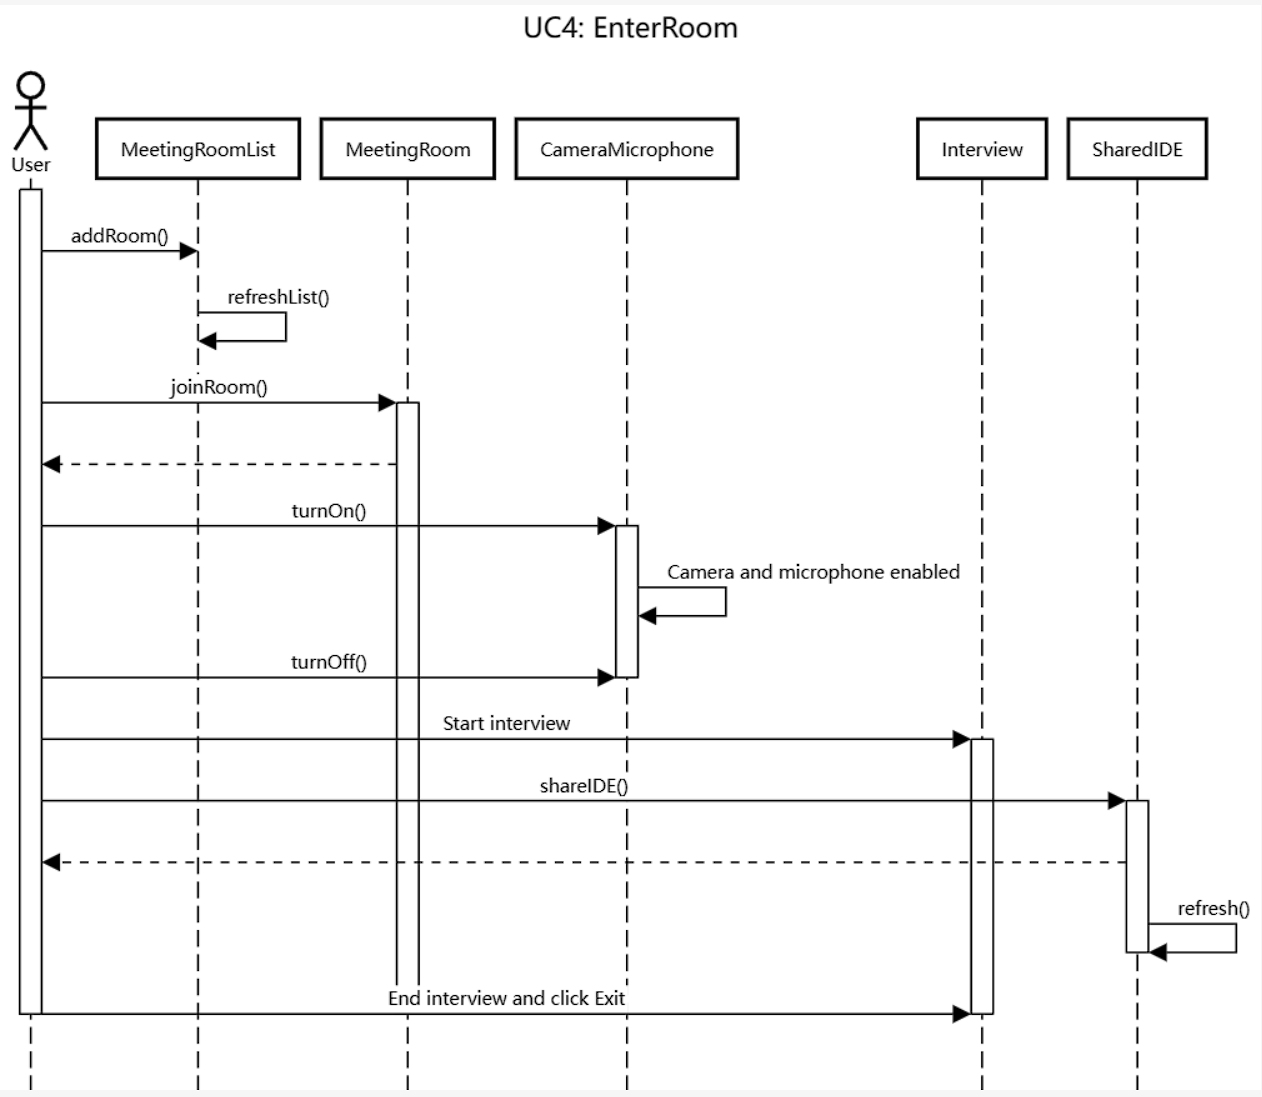
\includegraphics[scale=0.21]{diagrams/UC4.png}
  \caption{Use observer mode to check whether the user is in the meeting.}
\end{figure}


\begin{figure}[H]
  \center
  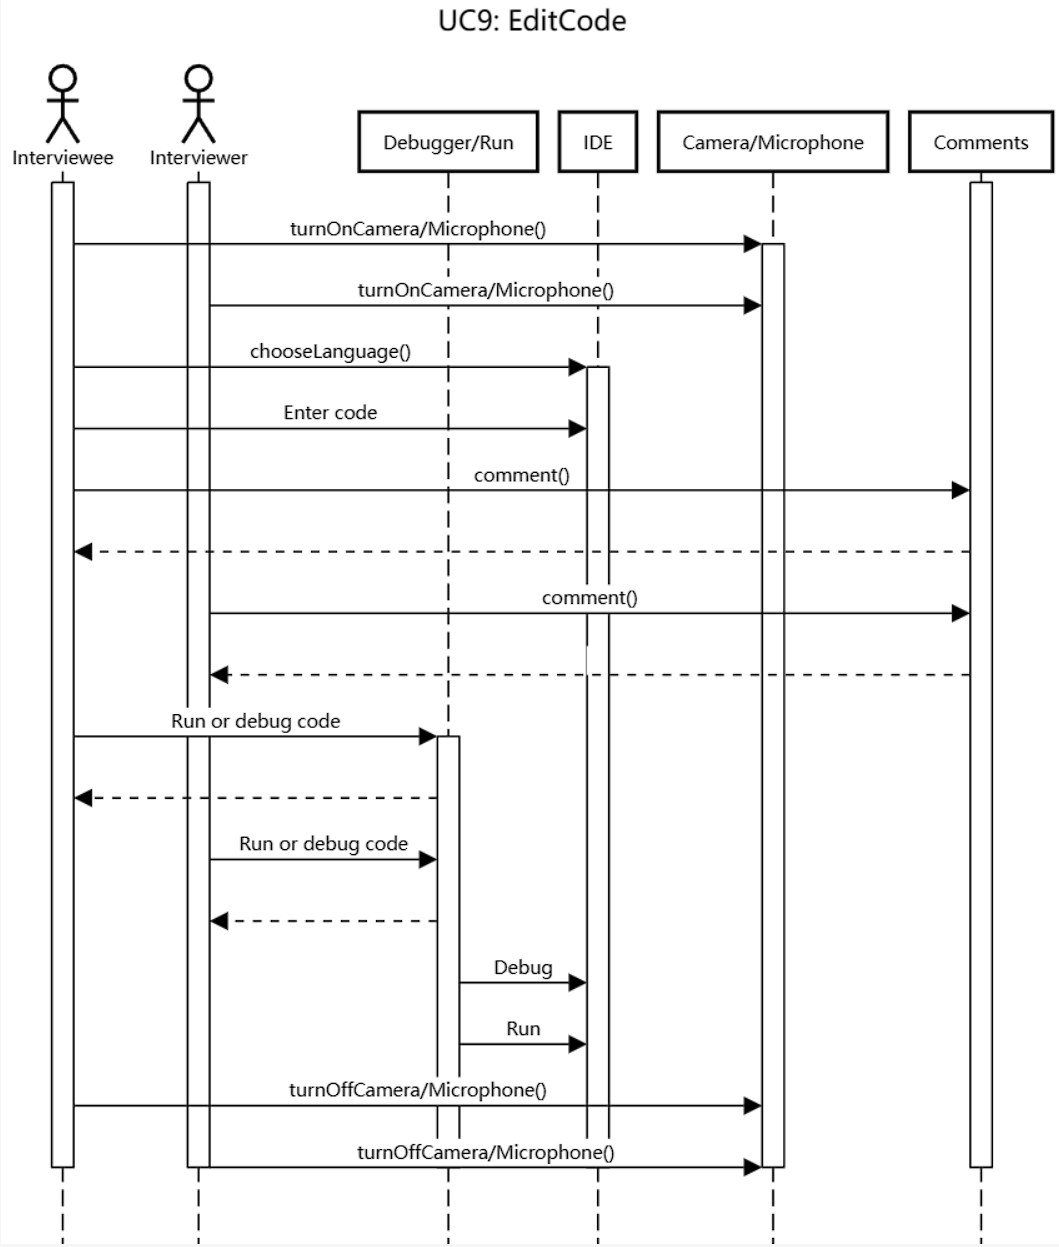
\includegraphics[scale=0.21]{diagrams/UC9.png}
  \caption{Use the chain of responsibility pattern to let the interviewer and the interviewer work with the same compiler and pass code.}
\end{figure}

\begin{figure}[H]
  \center
  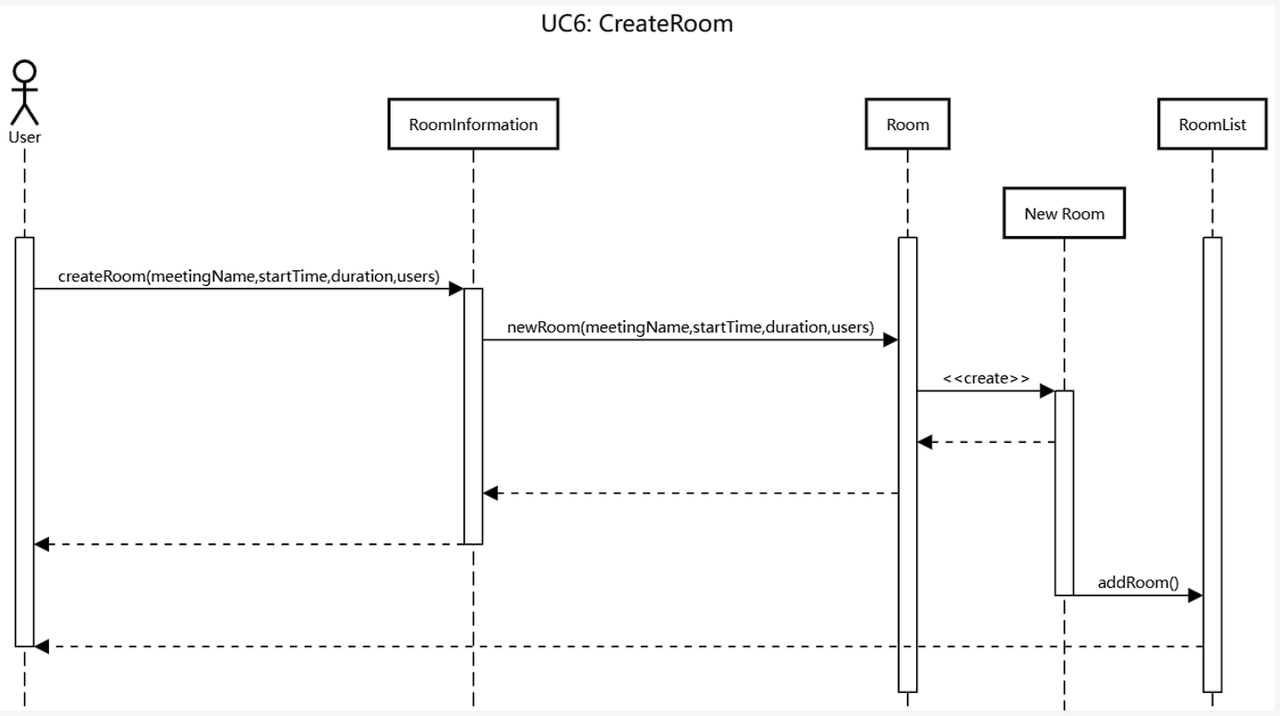
\includegraphics[scale=0.21]{diagrams/UC6.png}
  \caption{The meeting room is created using Builder mode.}
\end{figure}

\subsection{Class Diagram}

\begin{figure}[H]
  \center
  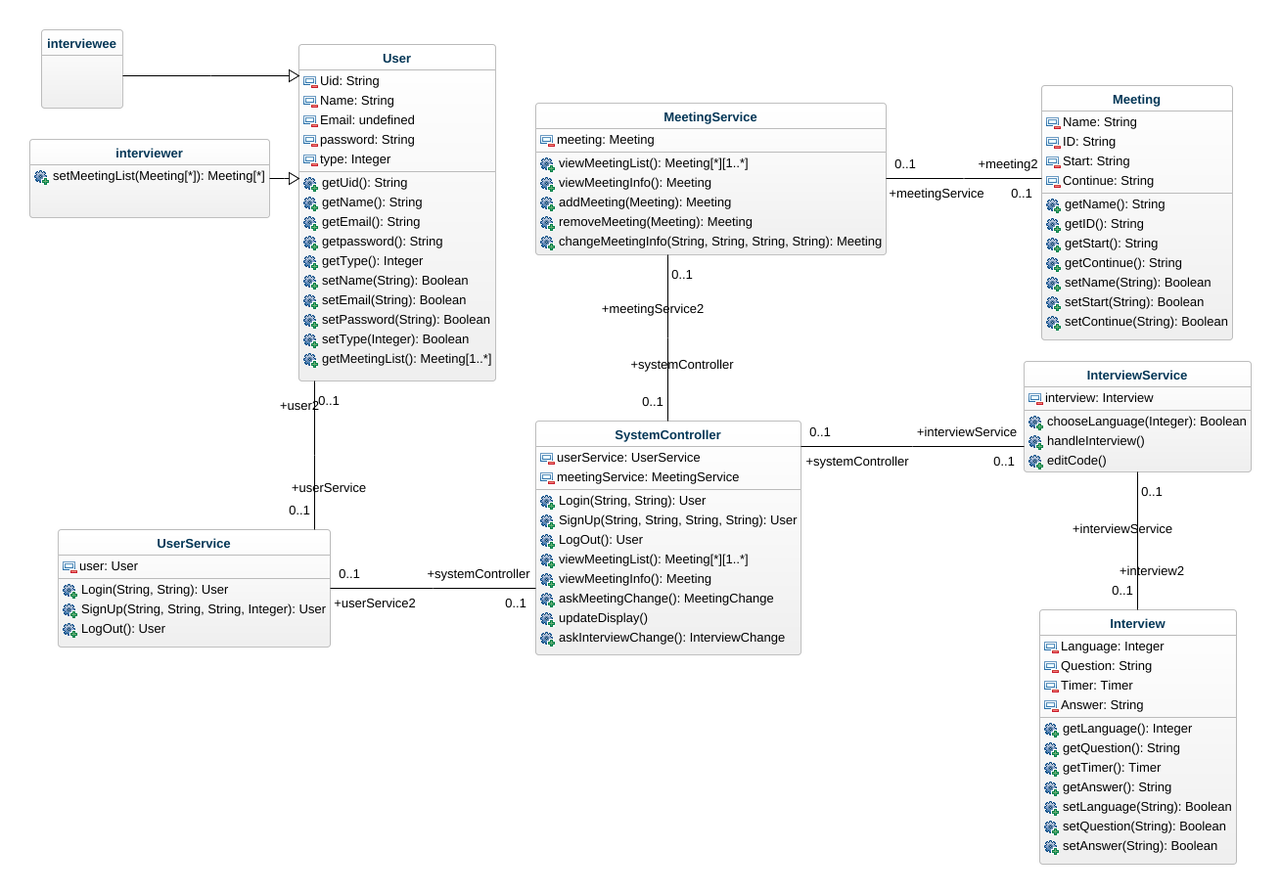
\includegraphics[scale=0.3]{diagrams/class-diagram.png}
  \caption{Class Diagram}
\end{figure}

\subsubsection*{Description of Responsibilities}

\begin{itemize}
  \item \textbf{Meeting:} The Meeting class is a basic entity class. Its attributes include name, id, start time, and duration continue. The Meeting class contains the following methods: geter() method for each attribute and seter() method for each attribute excluding ID.
  \item \textbf{MeetingService:} The MeetingService class is a basic entity class. Its properties are instance objects of the Meeting class. The MeetingService class includes the following methods: methods for browsing meeting lists, methods for browsing meeting information, methods for modifying meeting information, methods for adding and removing meetings.
  \item \textbf{User:} The User class is a basic entity class, which is the parent class of the Interviewee class and the Interviewer class. Its properties include uid, name, email, password and type filled in during registration, where type is used to distinguish whether the user is an internee or an internee. The User class contains the following methods: getter() and setter() methods for each attribute, and getMeetingList() methods for obtaining the meeting list.
  \item \textbf{Interviewee:} The Interviewee class is a basic entity class that is a subclass of the User class.
  \item \textbf{Interviewer:} The Interviewer class is a basic entity class that is a subclass of the User class. In addition to reusing all methods of the parent class, the Interviewer class also has the setMeetingList (Meeting [*]) method for creating a meeting list.
  \item \textbf{UserService:} The UserService class is a basic entity class. Its property is an instance object of the User class. The UserService class includes the following methods: registration and login for users when entering the application, as well as logout methods when exiting the application.
  \item \textbf{Interview:} The View class is a basic entity class. Its properties include programming language, question, answer duration timer, and answer. The Interview class contains the following methods: geter() methods for each property and seter() methods for each property that removes timers.
  \item \textbf{InterviewService:} The InterviewService class is a basic entity class. Its property is an instance object of the Interview class. The InterviewService class includes the following methods: the language selection method choseLanguage (Integer), and methods for managing interviews and editing code.
  \item \textbf{SystemController:} The SystemController class is a basic entity class. Its properties are instance objects of the UserService class and the MeetingService class. The SystemController class includes several methods: registration and login for users when entering the application, as well as logout methods when exiting the application. The browsing methods for meeting lists and meeting information. For the inquiry method modified during the meeting, for the inquiry method modified during the interview, and for updating the display method.
\end{itemize}

\subsection{System Architecture and System Design}

\subsubsection*{Architectural Styles}
\begin{itemize}
  \item \textbf{Frontend:} The front-end uses the React framework to generate SPA (Single Page Application), which requests the back-end to return JSON data and then renders it by the front-end framework. The front end uses tsx based on typescript to generate html templates, typescript is used to execute the script language and control the front-end logic, and moduleCSS+tailwindCSS is used to generate the style sheet. Use the webRTC interface that comes with the browser to read the audio and video streams. After entering the room, the front and back ends will use socket.io to establish a full-duplex P2P connection.
  \item \textbf{Backend:} The backend of the platform makes use of Flask as its framework to support all the functionalities, from creating an account to making a meeting appointment. It uses SQL Alchemy to make it easier and clearer to generate database models. 
\end{itemize}

\subsubsection*{UML Package Diagram of Subsystems}
\begin{figure}[H]
  \center
  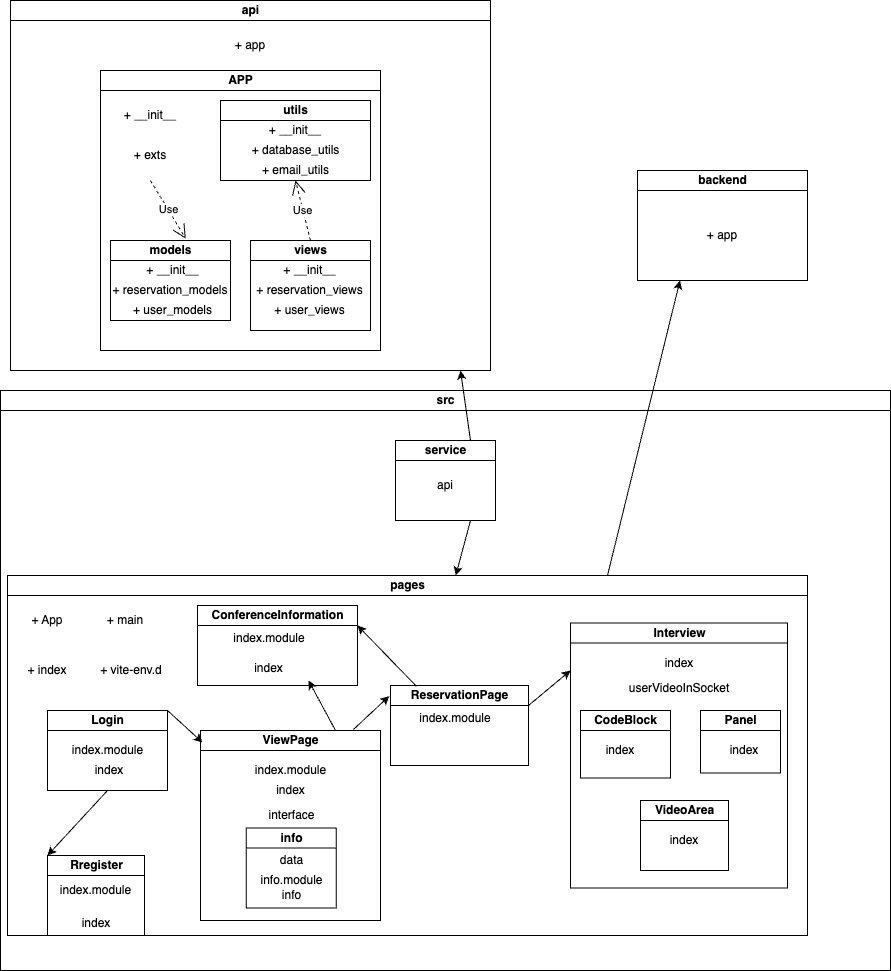
\includegraphics[scale=0.3]{diagrams/package-diagram.png}
  \caption{Package Diagram}
\end{figure}

\subsubsection*{Database Schema of the System}
There are three tables in the database: \verb|user|, \verb|reservation| and \verb|reservation\_participant|. The \verb|user| table is for storing data related to the user account of this platform (user ID, password, name, type of user, etc.), with \verb|user\_id| as its primary key, identifying each user. The \verb|reservation| table is for storing data related to the information of meetings. Its attributes involve the name, start time, end time, state, details and date of a meeting. The table uses an auto-increment ID serving as the primary key to identify each meeting. The \verb|reservation\_participant| table is a helper table for remembering the relationship of users and meetings, that is, the number of users involved in a meeting. It has an auto-increment ID as its primary key.

The design of the database meets the requirements of the Boyce-Codd normal form. Each table has a primary key, and all attributes in each table are functionally dependent on their respective primary keys, which are also superkeys. This eliminates redundancy and updates anomalies by ensuring every non-trivial functional dependency is on a superkey.

\subsubsection*{Global Control Flow of the System}
The user registers an account, and the system backend creates a new account and stores it in the database. When the user logs in, the backend verifies that the password is correct. If the password is incorrect, an error message is returned. If the password is correct, the user enters the main page.

On the main page, the system displays the user's nickname and identity, as well as a button to return to the login interface, displays user-related meeting information, and the interviewer additionally displays a button to schedule a meeting.

When the interviewer clicks the reservation button, the system will jump to the reservation page. The system will display the meeting-related information fill-in column. After the interviewer fills in the relevant information, click the reservation button to create the meeting. The system will navigate to the main meeting page and re-render the meeting information.

When the user clicks the meeting information icon, the system will jump to the meeting information page, where the system displays meeting-related information.

On the meeting information page, the interviewer clicks the Cancel Meeting button to cancel the meeting, and the system navigates to the main page and re-renders the meeting information.

On the meeting information page, the interviewer clicks the Edit meeting button to edit the meeting, and the system navigates to the reservation page. After the interviewer refills the information, the system navigates to the main page and re-renders the meeting information.

In the meeting information page, the user clicks the Enter meeting button, and the system navigates to the meeting page.

After clicking to join the interview, the backend will verify whether the user is in this interview. If not in the interview, the user is allowed to enter the interview room page.

After entering the interview room page, the interviewer/interviewer needs to click a button to turn on his or her camera and microphone.

If the network is normal, the connection will be established and the interviewer/interviewer can see the other party's ID, screen and share the IDE.

\subsubsection*{Hardware Requirements}
\begin{itemize}
  \item \textbf{Minimal configuration:} 
  \begin{enumerate}
    \item The device can run the chrome browser.
    \item The device can access the Internet (for P2P connection establishment)
  \end{enumerate}
  \item \textbf{Optimal configuration:} Available camera/microphone to enable video and audio streaming, called via Chrome browser.
\end{itemize}

\subsubsection*{Algorithms and Data Structures in the System: HashTable}
\begin{lstlisting}
// Save all connections
const clients = {};
setInterval(() => {
for (const client in clients) {
  clients[client].ws.emit('updateAllClients', {
    data: Object.keys(clients),
    })
  }
}, 2000)
\end{lstlisting}
User (client) related information, including socket instance object, room id and user id are stored in the clients object.

The key is the user's id, and the value is user-related information.
\begin{lstlisting}
switch (message.type) {
  case "connect":
    // Save the connected clients
    clientID = message.data.myID;
    roomID = message.data.roomID
    console.log(`${clientID} has connected in ${roomID}`)
    clients[clientID] = {
      clientID,
      roomID,
      ws,
    };
    ...
}
\end{lstlisting}
When a user initiates a video stream push to another user, the socket instance object of the other user is obtained through the clientID, and the emit method is called to trigger the event.

Using hashTable to store information makes the structure clear and improves access efficiency.

\subsection{Design of Tests}
\begin{enumerate}
  \item \textbf{Unit Testing:}
  \begin{itemize}
    \item Test Case 1: Browser-based IDE Functionality
    \begin{itemize}
      \item Description: Verify that the browser-based IDE allows candidates to write, execute, and debug code.
      \item Steps: 
      \begin{enumerate}
        \item Open the IDE
        \item Write code in different programming languages.
        \item Execute and debug code within the IDE.
        \item Ensure proper error handling.
      \end{enumerate}
    \end{itemize}
  \end{itemize}
  \begin{itemize}
    \item Test Case 2: Multi-language Support
    \begin{itemize}
      \item Description: Confirm that the platform supports multiple programming languages.
      \item Steps: 
      \begin{enumerate}
        \item Write and execute code in different programming languages.
        \item Verify language-specific features (e.g., syntax highlighting).
        \item Ensure smooth transitions between languages.
      \end{enumerate}
    \end{itemize}
  \end{itemize}
  \begin{itemize}
    \item Test Case 3: Video and Audio Interviewing
    \begin{itemize}
      \item Description: Test the functionality of video and audio interviewing.
      \item Steps: 
      \begin{enumerate}
        \item Initiate a video interview session.
        \item Confirm video and audio feeds are working.
        \item Test mute/unmute and video on/off functionalities.
        \item Verify the quality of audio and video.
      \end{enumerate}
    \end{itemize}
  \end{itemize}
  \begin{itemize}
    \item Test Case 4: Interview Scheduling and Management
    \begin{itemize}
      \item Description: Ensure interview scheduling and management features work correctly.
      \item Steps: 
      \begin{enumerate}
        \item Schedule an interview for a specific date and time.
        \item Confirm notifications are sent to interviewers and candidates.
        \item Check rescheduling and cancellation functionalities.
      \end{enumerate}
    \end{itemize}
  \end{itemize}
  \item \textbf{Test Coverage:}
  \begin{itemize}
    \item Aim to cover all critical functions of the browser-based IDE, video/audio interviewing and scheduling.
    \item Ensure each supported programming language is tested.
  \end{itemize}
  \item \textbf{Integration Testing Strategy:}
  \begin{itemize}
    \item Integrate components to ensure they work together seamlessly.
    \item Verify communication between the browser-based IDE, video and audio functions and scheduling features.
    \item Test the system's ability to handle multiple users in a live interview scenario.
  \end{itemize}
  \item \textbf{Integration Testing Plans:}
  \begin{itemize}
    \item Steps:
    \begin{enumerate}
      \item Conduct end-to-end testing of a complete interview session.
      \item Simulate concurrent users accessing the platform.
      \item Test interruptions and resume functionality during an ongoing interview.
      \item Check for compatibility with different browsers and devices.
    \end{enumerate}
  \end{itemize}
\end{enumerate}

\subsection{User Interface Design}


\subsubsection*{User Interface Description}

The user interface is divided into four main parts: \textit{Sign Up/Login}, \textit{Joining a Meeting}, \textit{Booking a Meeting}, and a \textit{Meeting Schedule}. The following descriptions provide a brief overview of each feature included and offer preliminary models of some key features.

\begin{itemize}
  \item \textbf{Joining a Meeting:} After clicking to join the meeting, the meeting details will be displayed in a pop-up window.
  \item \textbf{Meeting Schedule:} The meeting schedule contains the meetings that users will participate in in order of meeting start time. After clicking on any of the meetings, the meeting details will appear and the meeting details will be displayed in a pop-up window.
  \item \textbf{Meeting Details:} The content in this pop-up window includes: \textit{meeting name}, \textit{meeting duration}, \textit{start time and end time of the meeting}, \textit{initiator of this meeting}, \textit{canceling the meeting}, \textit{editing the meeting} and \textit{entering the meeting}. The user clicks \textit{Enter Meeting} in the pop-up window to enter the meeting room; or clicks the \textit{Return} button in the upper left corner to close the pop-up window. Only the meeting initiator is allowed to click the \textit{Cancel Meeting} and \textit{Edit Meeting} buttons below the pop-up window; invitees cannot click these two buttons. After clicking \textit{Cancel Meeting}, the meeting will be deleted; after clicking \textit{Edit Meeting}, the page will jump to the information filling page in the \textit{appointed meeting} for modification.
  \item \textbf{Booking a Meeting:} After clicking to schedule a meeting, the user needs to fill in the following information for this meeting in a new page: \textit{meeting name (the default name is "username's scheduled meeting")}, \textit{start time}, \textit{duration of the meeting (options are: 30min, 45min, 60min)} and \textit{the invitees}. This column requires an ID. The user clicks \textit{Complete Appointment} below the page to end information filling. After completed, the user will return to the main page and see the newly scheduled meeting in the \textit{Meeting Schedule} on the right side of the page.
\end{itemize}

\subsubsection*{User Interface Prototype}
\begin{figure}[H]
  \center
  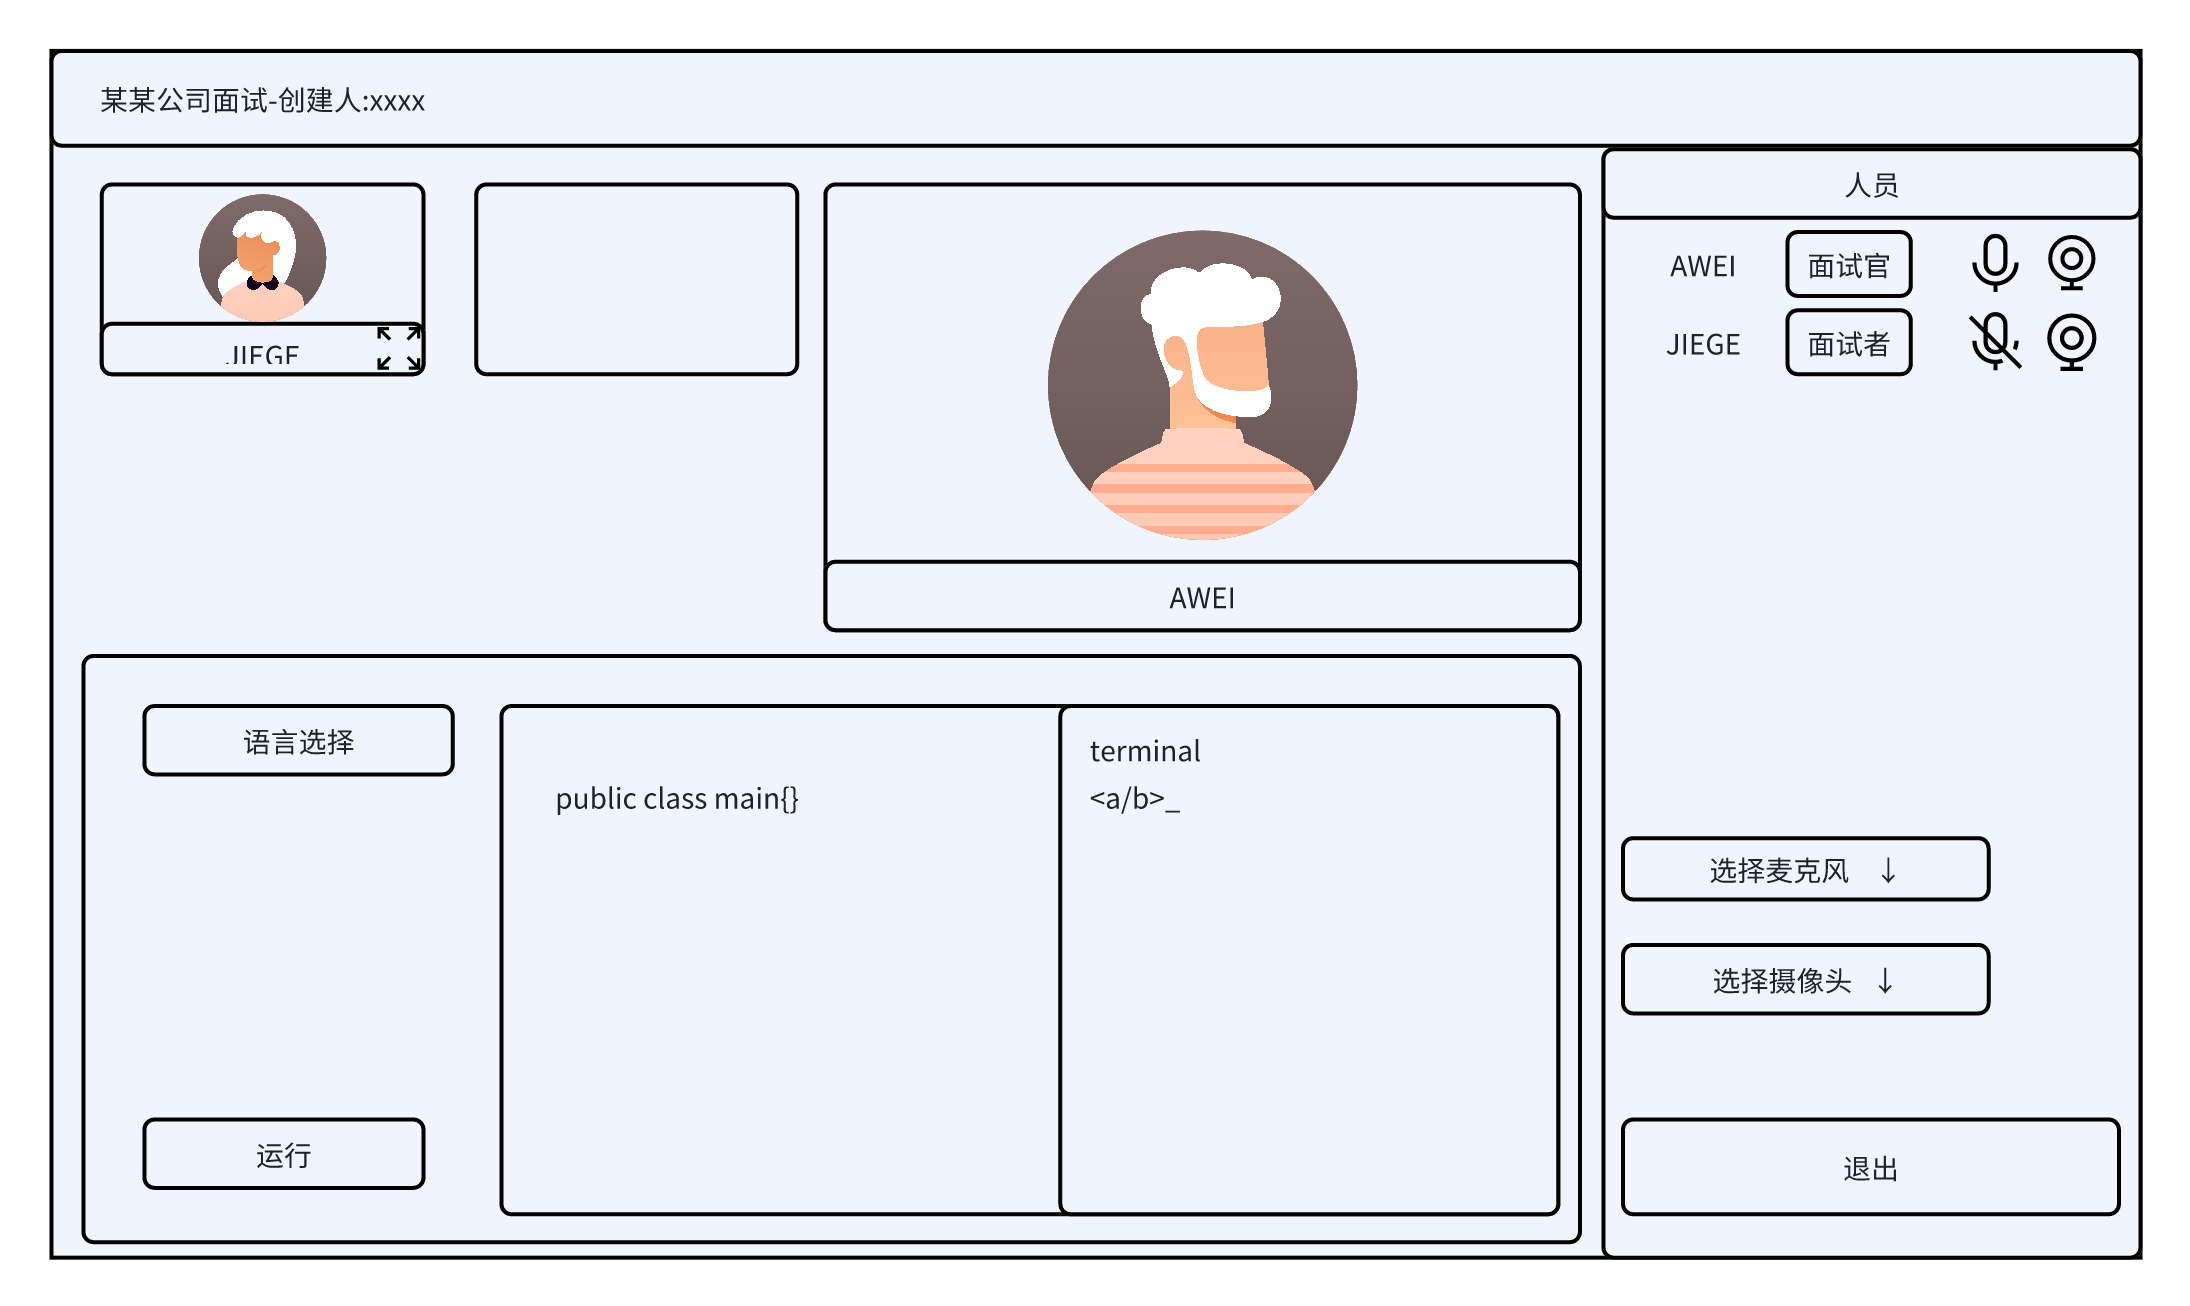
\includegraphics[scale=0.18]{diagrams/ui-prototype-1.png}
  \caption{UI Prototype 1}
\end{figure}

\newpage
\begin{figure}[H]
  \center
  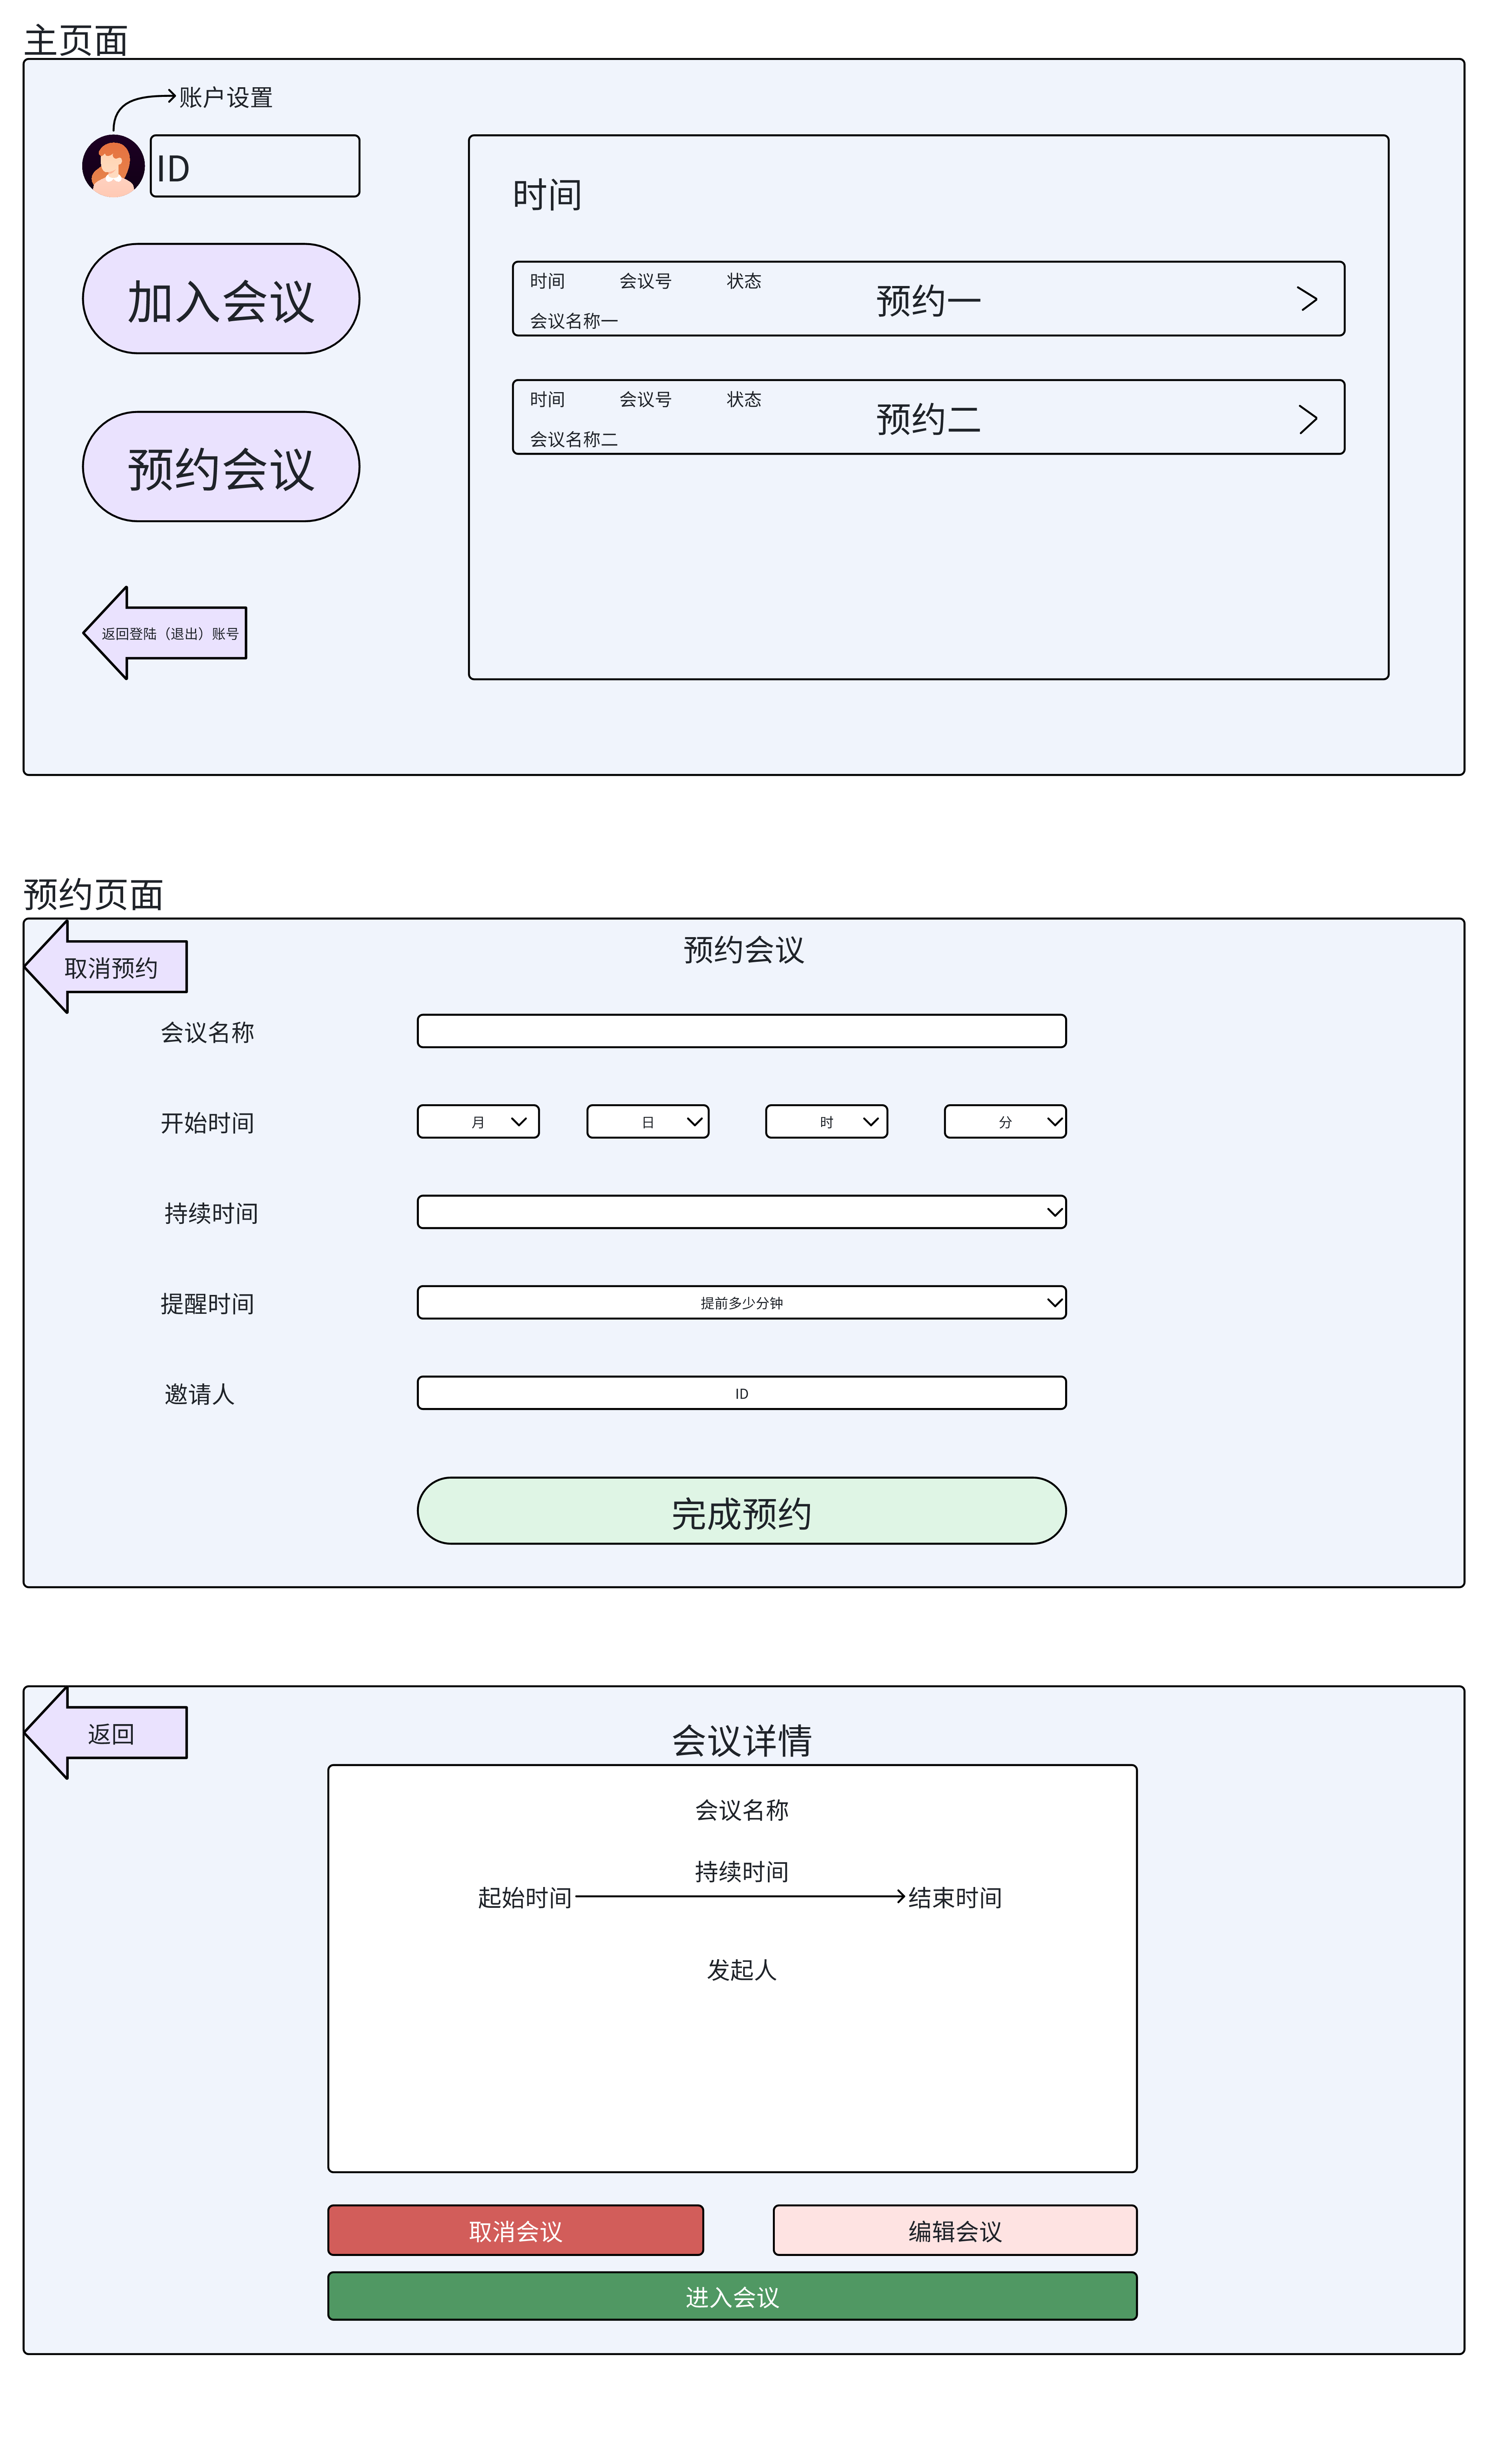
\includegraphics[scale=0.1]{diagrams/ui-prototype-2.png}
  \caption{UI Prototype 2}
\end{figure}

\section{Project Management}
\subsection{Team Agreement}
\begin{itemize}
  \item \textbf{Meeting Time:} Every Monday at 9pm and every Friday at 5pm.
  \item \textbf{Code Management:} This project uses git to manage the source code and other related resources. 
  A private repository on GitHub is used for hosting code and team collaboration. Commit message should be 
  clear and follow the convention like \par \verb|<type>[optional scope]: <description>|. Any changes that may be 
  deemed destructive should be made on a separate branch and then merged to the main branch after stabilized 
  and being reviewed by at least one other team member. All backend code should be tested using Apifox before 
  submitted.
  \begin{figure}[H]
    \center
    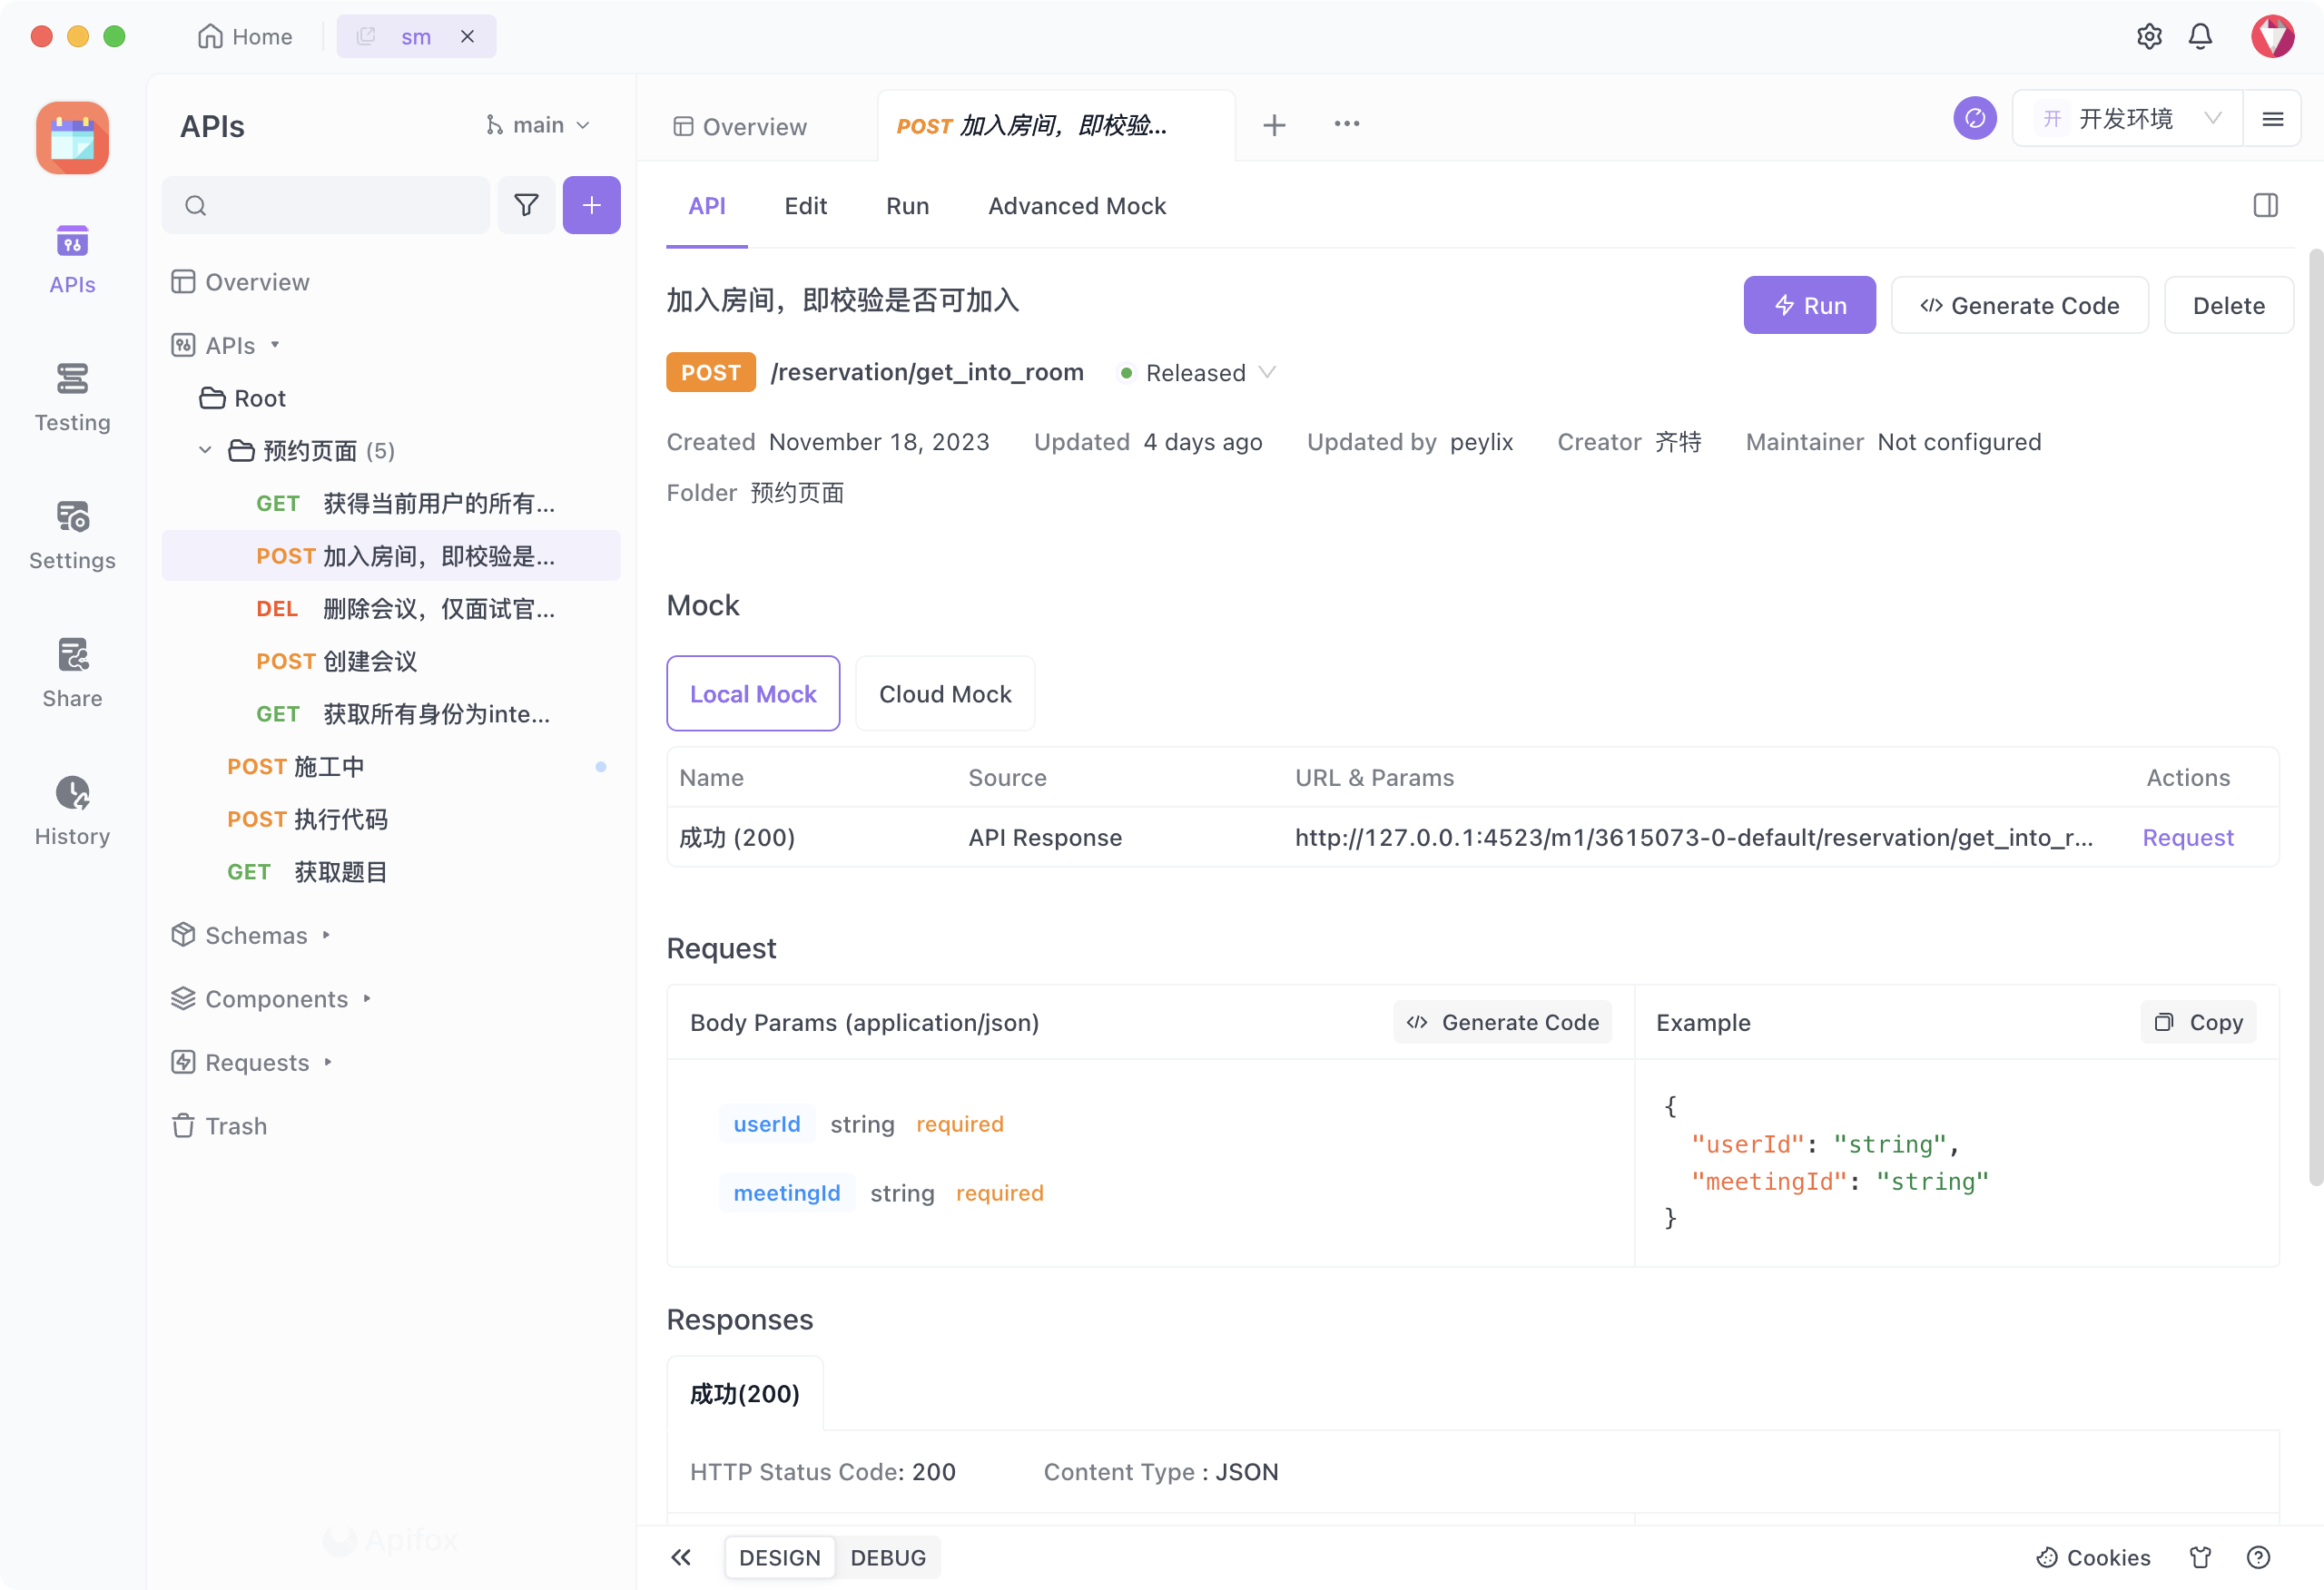
\includegraphics[scale=0.15]{diagrams/apifox.png}
    \caption{Using Apifox to test APIs}
  \end{figure}
  \item \textbf{Details for Cooperation:} A clear API document with detailed comments should be provided by the 
  team members who is responsible for the backend. The backend developers and frontend developers should work 
  closely together.
  \item \textbf{Overall Management:} In order to better manage tasks and project progress, a Gantt chart was 
  created so that the phased progress of the project and the task allocation of each member can be clearly seen. 
  Not only does this help track overall progress, but it also provides clear direction for team members so they can 
  better understand the overall framework of the project and their own roles.

  The Gantt chart can be found in 
  
  \url{https://cs9lscied6.feishu.cn/share/base/view/shrcnWfsEBhYGWS0lAVpVeuKQTd}
\end{itemize}

\subsection{Division of Work}
Frontend: 
\begin{itemize}
  \item Te Qi
  \item Tongyu Wu
  \item Jiehongxu Wu
\end{itemize}
Backend:
\begin{itemize}
  \item Sichen Li
  \item Ziqin Ma
\end{itemize}

The detailed division and contribution of each member is as follows:
\begin{figure}[H]
  \center
  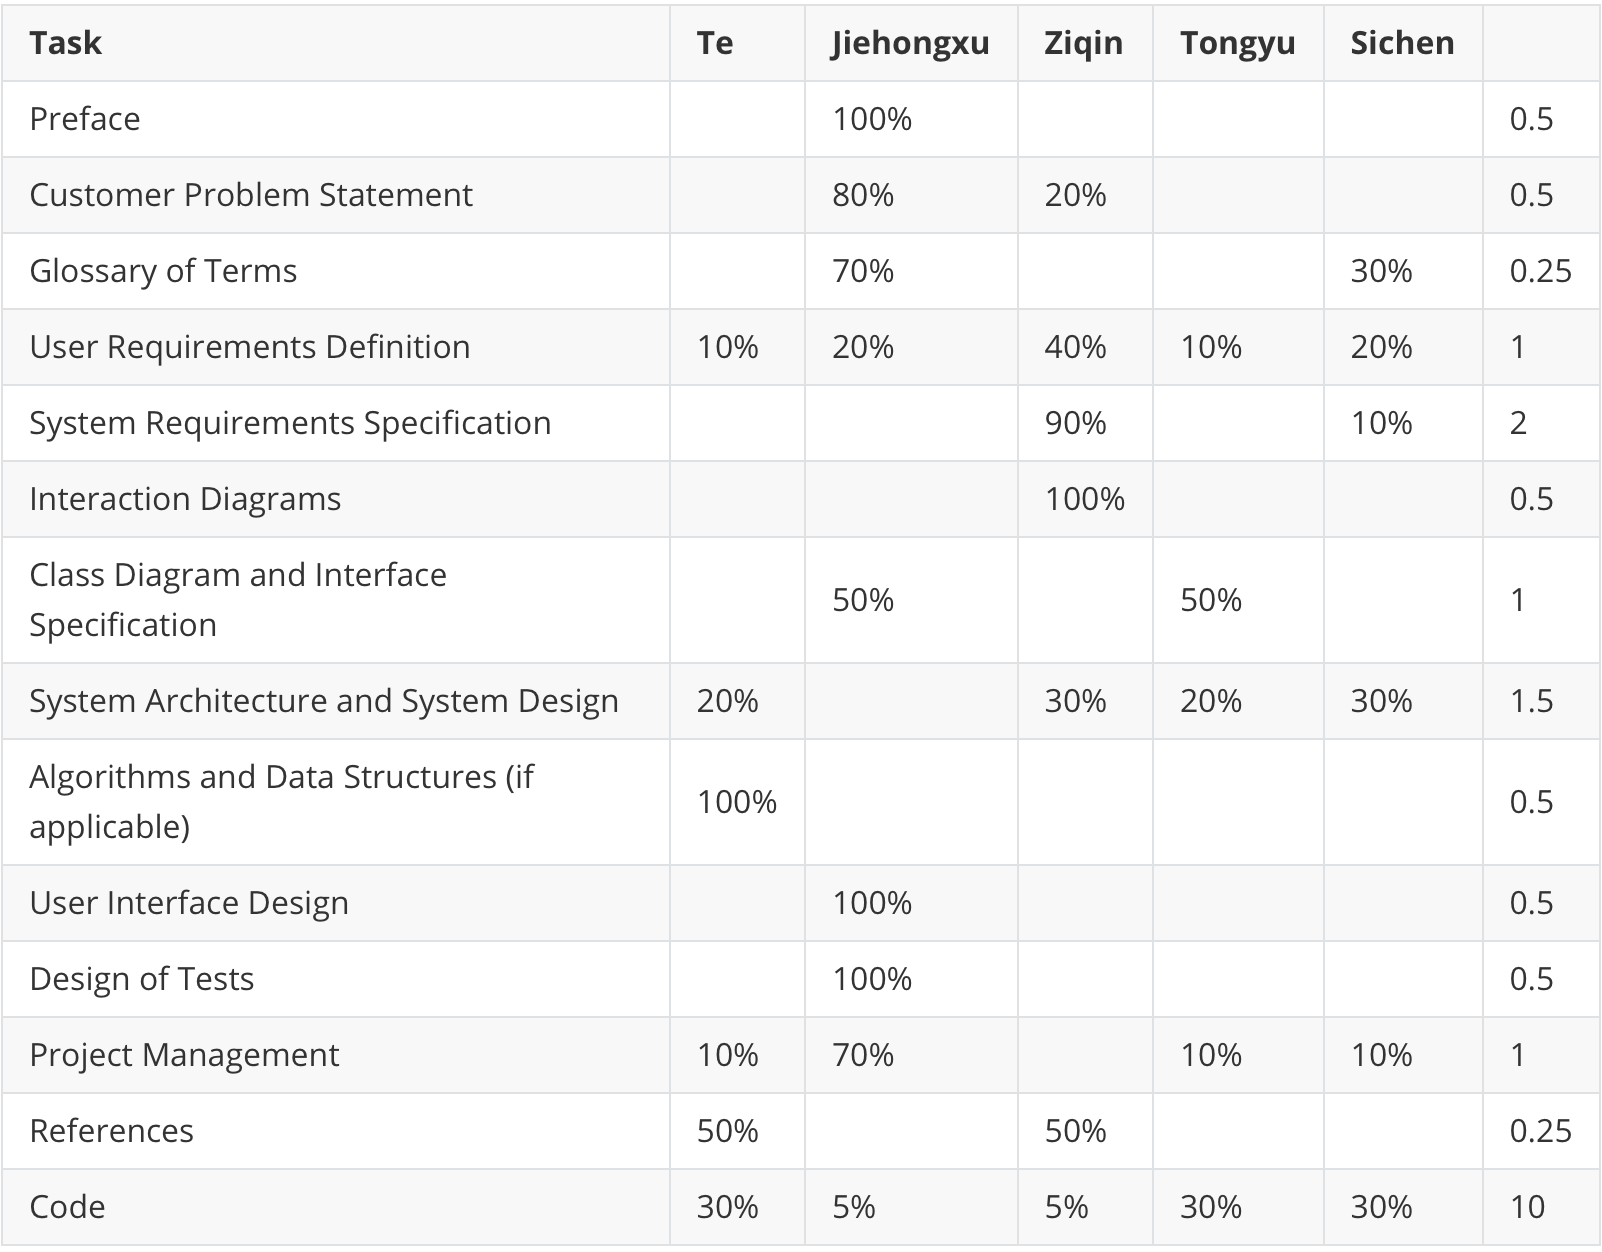
\includegraphics[scale=0.25]{diagrams/contribution.png}
\end{figure}

\end{document}
